\documentclass[11pt]{article}
\usepackage[margin=18mm,headheight=22pt]{geometry}
\usepackage{amsmath}
\usepackage{fontspec}
\usepackage{unicode-math}
\setmainfont{NewCM10}[Extension=.otf,UprightFont=*-Book,BoldFont=*-Bold,ItalicFont=*-BookItalic,BoldItalicFont=*-BoldItalic]
\setsansfont{NewCMSans10}[Extension=.otf,UprightFont=*-Book,BoldFont=*-Bold,ItalicFont=*-BookOblique,BoldItalicFont=*-BoldOblique]
\setmathfont{NewCMMath-Book.otf}
\usepackage{xcolor}
\definecolor{FAUblue}{HTML}{04316A}
\definecolor{Paperblue}{HTML}{EEF2F7}
\definecolor{EEIgold}{HTML}{CC9C42}
\usepackage{etoolbox,enumitem,booktabs,tabularx,array,needspace,microtype}
\usepackage[most]{tcolorbox}
\usepackage{titlesec,fancyhdr}
\usepackage[hidelinks]{hyperref}
\usepackage{draftwatermark}
\SetWatermarkText{Made by Thanate Amornjiraporn (Focus)}
\SetWatermarkColor{black!7}\SetWatermarkFontSize{30pt}\SetWatermarkAngle{45}
\setlength{\parindent}{0pt}
\setlength{\parskip}{5pt}
\setlist{itemsep=2pt,topsep=3pt,leftmargin=1.6em,beginpenalty=10000,endpenalty=10000}
\raggedbottom
\clubpenalty=10000 \widowpenalty=10000 \displaywidowpenalty=10000 \interlinepenalty=10000
\setcounter{secnumdepth}{0}
\setcounter{tocdepth}{1}
\pagestyle{fancy}\fancyhf{}
\fancyhead[L]{\small\sffamily\color{FAUblue} From Fundamentals to AI Apocalypse · MEI · Chapter 4}
\fancyhead[R]{\small\sffamily Complex Numbers}
\fancyfoot[C]{\small\thepage}
\titleformat{\section}{\Large\bfseries\sffamily\color{FAUblue}}{}{0pt}{}
\titleformat{\subsection}{\large\bfseries\sffamily\color{FAUblue}}{}{0pt}{}
\titlespacing*{\section}{0pt}{16pt}{6pt}
\preto\section{\Needspace{8\baselineskip}}
\preto\subsection{\Needspace{6\baselineskip}}
\newtcolorbox{equationcard}[1]{colback=Paperblue,colframe=Paperblue,boxrule=0pt,arc=0pt,left=10pt,right=10pt,top=6pt,bottom=6pt,title={#1},fonttitle=\small\bfseries\sffamily,coltitle=FAUblue,before skip=8pt,after skip=8pt}
\newtcolorbox{workedbox}[1]{colback=white,colframe=EEIgold,boxrule=0pt,leftrule=3pt,arc=0pt,left=10pt,top=4pt,bottom=4pt,title={#1},fonttitle=\small\bfseries\sffamily,coltitle=FAUblue,attach title to upper={\par},before skip=8pt,after skip=8pt}
\newtcolorbox{recallbox}[1]{colback=white,colframe=FAUblue,boxrule=0pt,leftrule=3pt,arc=0pt,left=10pt,top=4pt,bottom=4pt,title={#1},fonttitle=\small\bfseries\sffamily,coltitle=FAUblue,attach title to upper={\par},before skip=8pt,after skip=8pt}
\usepackage{environ}
\newsavebox\measurebox
% Typeset the section once invisibly to measure it; start a new page if it will not fit in what is left.
\makeatletter
\newif\ifkeep@measuring
\NewEnviron{keepsection}{%
  \ifkeep@measuring \BODY \else
    \edef\keep@sec{\the\value{section}}\edef\keep@sub{\the\value{subsection}}%
    \setbox\measurebox\vbox{\hsize\linewidth\keep@measuringtrue\def\Needspace##1{}\BODY}%
    \setcounter{section}{\keep@sec}\setcounter{subsection}{\keep@sub}%
    \dimen2=\ht\measurebox \advance\dimen2\dp\measurebox
    \dimen@=\textheight
    \ifdim\pagegoal<\maxdimen
      \dimen@=\pagegoal \advance\dimen@-\pagetotal
      \ifdim\dimen2>\dimen@ \clearpage \dimen@=\textheight \fi
    \fi
    % if it fits, nothing inside may force an early break
    \ifdim\dimen2>\dimen@ \BODY \else \begingroup\def\Needspace##1{}\BODY\endgroup \fi
  \fi}
\makeatother
\newtcolorbox{notebox}{colback=Paperblue,colframe=Paperblue,boxrule=0pt,arc=0pt,left=8pt,right=8pt,top=4pt,bottom=4pt,before skip=6pt,after skip=6pt}
\newtcolorbox{plainbox}{colback=white,colframe=FAUblue,boxrule=0pt,leftrule=3pt,arc=0pt,left=10pt,right=8pt,top=4pt,bottom=4pt,before skip=6pt,after skip=8pt}
\usetikzlibrary{arrows.meta}
\title{\sffamily\bfseries\color{FAUblue}Complex Numbers}
\author{Mathematics for Engineers I \ensuremath{\cdot} Module 27651 \ensuremath{\cdot} Chapter 4\\[2pt]\small From Fundamentals to AI Apocalypse · personal study guide}
\date{}
\begin{document}
\maketitle
\begingroup\footnotesize\setlength{\parskip}{0pt}\tableofcontents\endgroup
\clearpage

\Needspace{9\baselineskip}
{\large This chapter extends the number line to a plane, so that equations such as \textit{z}\textsuperscript{2} = \ensuremath{-}1 have solutions. You learn to calculate in normal and polar form, raise to powers and take roots, and meet the complex polynomial, exponential, logarithm, sine and cosine.}


\begin{keepsection}
\Needspace{17\baselineskip}
\section{Start from memory}

\Needspace{14\baselineskip}
Try these before reading. Write an answer even if you are uncertain; the gap tells you what to look for.

\Needspace{11\baselineskip}
\begin{enumerate}
\item Which number squares to \ensuremath{-}1, and what is it called?
\item How do you add two complex numbers?
\item What is the distance of 3+4i from the origin?
\item When you multiply two complex numbers, what happens to their lengths and their angles?
\item How many solutions does \textit{w}\textsuperscript{\textit{n}} = \textit{z} have when \textit{z} \ensuremath{\neq} 0?
\item If a polynomial with real coefficients has the zero 2+i, which other number must also be a zero?
\end{enumerate}

\nopagebreak[4]{\small\itshape Answers: see “Start from memory” under Answers at the end.}
\end{keepsection}

\begin{keepsection}
\Needspace{21\baselineskip}
\section{How to use this guide}

\Needspace{18\baselineskip}
Attempt each worked example before reading its steps. Then hide the guide and retrieve the method on a later day.

\Needspace{15\baselineskip}
\begin{enumerate}
\item \textbf{Day 0:} Do the cold start. Read §4.1 up to conjugate and magnitude, and plot five numbers of your own in the Gaussian plane.
\item \textbf{Day 1:} Finish §4.1 (polar form and polar multiplication). Rebuild the division and polar worked examples from a blank page, then try mixed practice 1–8.
\item \textbf{Day 3:} Study §4.2. Derive the n-th root formula cold, then solve practice 9–16 without notes.
\item \textbf{About day 7:} Study §4.3. Shuffle practice 17–24 and say aloud, for each, whether normal or polar form is the better tool.
\item \textbf{About day 14:} Rebuild every derivation in “Derive it cold” and retry every question you marked. Tick the self-check only with evidence from unaided work.
\item \textbf{Before the exam:} Do both exam problems under the time limit, then review only the skills your evidence shows are weak.
\end{enumerate}
\end{keepsection}

\begin{keepsection}
\Needspace{22\baselineskip}
\section{How the chapter fits together}

\Needspace{19\baselineskip}
A complex number is a point in a plane. Normal form describes it by its coordinates, polar form by its length and angle. Polar form turns multiplication into adding angles, which gives powers and roots; the exponential, logarithm, sine and cosine then extend to complex inputs through Euler’s formula.

\Needspace{9\baselineskip}
\subsection{Measured \ensuremath{\cdot} the number and its picture}

\Needspace{6\baselineskip}
\begin{itemize}
\item \Needspace{4\baselineskip}
\textbf{Normal form} \hfill{\small\color{FAUblue}§4.1}

\Needspace{4\baselineskip}
z = a + ib, i\textsuperscript{2} = \ensuremath{-}1

Rests on: the real numbers plus one new number i whose square is \ensuremath{-}1.
\item \Needspace{4\baselineskip}
\textbf{Gaussian plane} \hfill{\small\color{FAUblue}§4.1}

\Needspace{4\baselineskip}
a + ib = (a, b)

Rests on: reading the real and imaginary parts as coordinates.
\end{itemize}

\Needspace{11\baselineskip}
\subsection{Defined \ensuremath{\cdot} length, angle and functions}

\Needspace{8\baselineskip}
\begin{itemize}
\item \Needspace{4\baselineskip}
\textbf{Conjugate and magnitude} \hfill{\small\color{FAUblue}§4.1}

\Needspace{4\baselineskip}
|z|\textsuperscript{2} = z z̅

Rests on: reflection in the real axis and Pythagoras in the plane.
\item \Needspace{4\baselineskip}
\textbf{Polar and exponential form} \hfill{\small\color{FAUblue}§4.1}

\Needspace{4\baselineskip}
z = |z|e\textsuperscript{iφ}

Rests on: length |z| and angle φ, joined by Euler’s formula.
\item \Needspace{4\baselineskip}
\textbf{Complex exponential} \hfill{\small\color{FAUblue}§4.3}

\Needspace{4\baselineskip}
e\textsuperscript{x+iy} = e\textsuperscript{x}e\textsuperscript{iy}

Rests on: Euler’s formula for the angle and the real exponential for the length.
\end{itemize}

\Needspace{12\baselineskip}
\subsection{Derived \ensuremath{\cdot} results you calculate with}

\Needspace{9\baselineskip}
\begin{itemize}
\item \Needspace{4\baselineskip}
\textbf{Powers (de Moivre)} \hfill{\small\color{FAUblue}§4.2}

\Needspace{4\baselineskip}
z\textsuperscript{k} = |z|\textsuperscript{k}e\textsuperscript{ikφ}

Rests on: multiplying lengths and adding angles k times.
\item \Needspace{4\baselineskip}
\textbf{n-th roots} \hfill{\small\color{FAUblue}§4.2}

\Needspace{4\baselineskip}
w\textsubscript{k} = |z|\textsuperscript{1/\textit{n}}e\textsuperscript{i(φ+2kπ)/n}

Rests on: de Moivre run backwards, with angles known only up to 2π.
\item \Needspace{4\baselineskip}
\textbf{Factorising polynomials} \hfill{\small\color{FAUblue}§4.3}

\Needspace{4\baselineskip}
P(z) = a\textsubscript{n}(z \ensuremath{-} z\textsubscript{1})…(z \ensuremath{-} z\textsubscript{n})

Rests on: every polynomial having all its zeros in \ensuremath{\mathbb{C}}.
\item \Needspace{4\baselineskip}
\textbf{Complex logarithm} \hfill{\small\color{FAUblue}§4.3}

\Needspace{4\baselineskip}
ln z = ln|z| + iφ

Rests on: inverting e\textsuperscript{z} on a strip of height 2π.
\end{itemize}

\begin{keepsection}
\Needspace{18\baselineskip}
\subsection{Choose a tool}

\Needspace{10\baselineskip}
\begin{center}\small\begin{tabularx}{\linewidth}{>{\raggedright\arraybackslash}X>{\raggedright\arraybackslash}X}\toprule
\textbf{If the task asks…} & \textbf{Choose this tool} \\ \midrule
Add, subtract or simplify a quotient & Normal form; for a quotient, multiply top and bottom by the conjugate of the denominator. \\
Multiply, divide or raise to a power & Polar or exponential form: multiply lengths, add angles; de Moivre for powers. \\
Solve \textit{w}\textsuperscript{\textit{n}} = \textit{z} & The n-th root formula: n answers evenly spaced on a circle. \\
Describe a set of points & Distance |\textit{z} \ensuremath{-} \textit{a}| for circles and discs. \\
Factor a polynomial or find its zeros & Fundamental theorem of algebra; with real coefficients, zeros come in conjugate pairs. \\
Evaluate e\textsuperscript{\textit{z}}, ln \textit{z}, sin \textit{z} or cos \textit{z} & The definitions of §4.3, with the angle of ln \textit{z} taken in [0, 2π). \\
\bottomrule\end{tabularx}\end{center}
\end{keepsection}
\end{keepsection}

\begin{keepsection}
\Needspace{13\baselineskip}
\section{4.1 Definitions and Basic Arithmetic Operations}

\Needspace{10\baselineskip}
No real number squares to \ensuremath{-}1, so an equation as simple as \textit{z}\textsuperscript{2} + 1 = 0 has no real solution. Adding one new number and reading numbers as points of a plane fixes this, and every rule of real arithmetic still holds.

\begin{plainbox}\textbf{In plain words:} picture a complex number as a point on a map, with east–west as one direction and north–south as the other. The new ingredient is the \textbf{imaginary unit} i, a number whose square is \ensuremath{-}1. Writing a number as “a plus i times b” is its \textbf{normal form}; a is its \textbf{real part} and b its \textbf{imaginary part}, and the map that holds these points is the \textbf{Gaussian plane}. You can also give a point by how far it is from the origin and in which direction: that is the \textbf{polar form}.\end{plainbox}

\begin{keepsection}
\Needspace{11\baselineskip}
\subsection{Normal form and the Gaussian plane}

\begin{equationcard}{Normal form}
\[ \begin{gathered} {z}\, =\, {a}\, +\, \mathrm{i}{b} \\ \text{Re}\, {z}\, =\, {a},\, \text{Im}\, {z}\, =\, {b} \\ \mathrm{i}^{2}\, =\, -1 \end{gathered} \]
{\small \emph{Read it as: “z is a plus i b; a is the real part of z and b its imaginary part”.}\par Here \textit{a}, \textit{b} \ensuremath{\in} \ensuremath{\mathbb{R}}, and the number is the ordered pair (\textit{a}, \textit{b}). A real number \textit{x} is the complex number (\textit{x}, 0). Two complex numbers are equal exactly when their real parts and their imaginary parts are equal. \ensuremath{\mathbb{C}} is a field, but it has no order: “\textit{z} \ensuremath{<} \textit{w}” means nothing.}
\end{equationcard}

\Needspace{14\baselineskip}
\begin{center}
\begin{minipage}[t]{0.950\linewidth}\centering
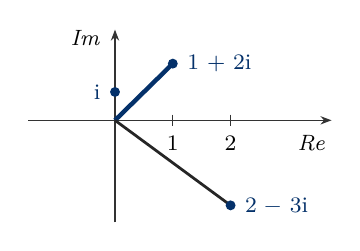
\begin{tikzpicture}[line join=round]
\draw[-{Stealth[length=4pt]},black!80] (0.720,-1.332) -- (4.572,-1.332);
\draw[-{Stealth[length=4pt]},black!80] (1.822,-2.628) -- (1.822,-0.180);
\draw[FAUblue,line width=1.6pt] (1.822,-1.332) -- (2.556,-0.612);
\draw[black!85,line width=1pt] (1.822,-1.332) -- (3.290,-2.412);
\fill[FAUblue] (2.556,-0.612) circle (0.063);
\node[anchor=west,text=FAUblue,fill=white,fill opacity=0.85,text opacity=1,inner sep=1pt,font=\footnotesize] at (2.700,-0.612) {1 + 2i};
\fill[FAUblue] (3.290,-2.412) circle (0.063);
\node[anchor=west,text=FAUblue,fill=white,fill opacity=0.85,text opacity=1,inner sep=1pt,font=\footnotesize] at (3.434,-2.412) {2 \ensuremath{-} 3i};
\fill[FAUblue] (1.822,-0.972) circle (0.063);
\node[anchor=east,text=FAUblue,fill=white,fill opacity=0.85,text opacity=1,inner sep=1pt,font=\footnotesize] at (1.678,-0.972) {i};
\node[anchor=east,inner sep=1pt,font=\footnotesize] at (4.536,-1.620) {\textit{Re}};
\node[anchor=east,inner sep=1pt,font=\footnotesize] at (1.678,-0.288) {\textit{Im}};
\draw[black!80] (2.556,-1.260) -- (2.556,-1.404);
\node[,inner sep=1pt,font=\footnotesize] at (2.556,-1.620) {1};
\draw[black!80] (3.290,-1.260) -- (3.290,-1.404);
\node[,inner sep=1pt,font=\footnotesize] at (3.290,-1.620) {2};
\end{tikzpicture}\par\smallskip{\small\raggedright \textbf{The Gaussian plane.} The real part is read along the horizontal axis and the imaginary part up the vertical axis: 1 + 2i sits at (1, 2), 2 \ensuremath{-} 3i at (2, \ensuremath{-}3) and i at (0, 1).\par}\end{minipage}
\end{center}

Engineers often write j for the imaginary unit, because i (or I) already stands for current. The notes use i; in a circuit calculation, check which letter means what.
\end{keepsection}

\begin{keepsection}
\Needspace{11\baselineskip}
\subsection{Calculating in normal form}

\begin{equationcard}{Sum, difference and product}
\[ \begin{gathered} ({a}_{1}\, +\, \mathrm{i}{b}_{1})\, \pm \, ({a}_{2}\, +\, \mathrm{i}{b}_{2})\, =\, ({a}_{1}\, \pm \, {a}_{2})\, +\, \mathrm{i}({b}_{1}\, \pm \, {b}_{2}) \\ ({a}_{1}\, +\, \mathrm{i}{b}_{1})({a}_{2}\, +\, \mathrm{i}{b}_{2})\, =\, ({a}_{1}{a}_{2}\, -\, {b}_{1}{b}_{2})\, +\, \mathrm{i}({a}_{1}{b}_{2}\, +\, {b}_{1}{a}_{2}) \end{gathered} \]
{\small \emph{Read it as: “add real parts to real parts and imaginary parts to imaginary parts”; for the product, “multiply out as with real numbers and replace i squared by \ensuremath{-}1”.}\par Adding and subtracting work like vectors in the plane.}
\end{equationcard}

\begin{equationcard}{Quotient}
\[ \begin{gathered} \dfrac{{z}}{{w}}\, =\, \dfrac{({a}_{1}\, +\, \mathrm{i}{b}_{1})({a}_{2}\, -\, \mathrm{i}{b}_{2})}{({a}_{2}\, +\, \mathrm{i}{b}_{2})({a}_{2}\, -\, \mathrm{i}{b}_{2})}\, =\, \dfrac{{a}_{1}{a}_{2}\, +\, {b}_{1}{b}_{2}}{{a}_{2}^{2}\, +\, {b}_{2}^{2}}\, -\, \mathrm{i}\dfrac{{a}_{1}{b}_{2}\, -\, {b}_{1}{a}_{2}}{{a}_{2}^{2}\, +\, {b}_{2}^{2}} \\ \dfrac{1}{{a}\, +\, \mathrm{i}{b}}\, =\, \dfrac{{a}\, -\, \mathrm{i}{b}}{{a}^{2}\, +\, {b}^{2}} \end{gathered} \]
{\small \emph{Read it as: “multiply top and bottom by the conjugate of the bottom”.}\par Valid for \textit{w} \ensuremath{\neq} 0. The bottom becomes (\textit{a} + i\textit{b})(\textit{a} \ensuremath{-} i\textit{b}) = \textit{a}\textsuperscript{2} + \textit{b}\textsuperscript{2}, a real number. In particular {\small\ensuremath{\dfrac{1}{\mathrm{i}}}} = \ensuremath{-}i.}
\end{equationcard}

\Needspace{12\baselineskip}
Multiplying by i turns a point a quarter turn counterclockwise about the origin: i(\textit{a} + i\textit{b}) = \ensuremath{-}\textit{b} + i\textit{a}. Multiplying by i four times brings you back, since i\textsuperscript{4} = 1.

\begin{workedbox}{Worked example \ensuremath{\cdot} the four operations}
Let \textit{z} = 3 + i and \textit{w} = 1 \ensuremath{-} 2i.

\Needspace{6\baselineskip}
\begin{enumerate}
\item Sum and difference, part by part: \textit{z} + \textit{w} = 4 \ensuremath{-} i and \textit{z} \ensuremath{-} \textit{w} = 2 + 3i.
\item Product: (3 + i)(1 \ensuremath{-} 2i) = 3 \ensuremath{-} 6i + i \ensuremath{-} 2i\textsuperscript{2} = 3 \ensuremath{-} 5i + 2 = 5 \ensuremath{-} 5i.
\item Quotient: multiply top and bottom by 1 + 2i. The bottom is 1\textsuperscript{2} + 2\textsuperscript{2} = 5 and the top is (3 + i)(1 + 2i) = 3 + 6i + i + 2i\textsuperscript{2} = 1 + 7i, so {\small\ensuremath{\dfrac{{z}}{{w}}}} = {\small\ensuremath{\dfrac{1}{5}}} + {\small\ensuremath{\dfrac{7}{5}}}i.
\end{enumerate}

Check the quotient by multiplying back: (1 \ensuremath{-} 2i)(1 + 7i) = 1 + 7i \ensuremath{-} 2i \ensuremath{-} 14i\textsuperscript{2} = 15 + 5i, and dividing by 5 gives 3 + i = \textit{z}.
\end{workedbox}
\end{keepsection}

\begin{keepsection}
\Needspace{11\baselineskip}
\subsection{Conjugate, magnitude and distance}

\begin{equationcard}{Conjugate and magnitude}
\[ \begin{gathered} {\overline{z}}\, =\, {a}\, -\, \mathrm{i}{b} \\ |{z}|\, =\, \sqrt{{a}^{2}\, +\, {b}^{2}} \\ |{z}|^{2}\, =\, {z}\, \cdot \, {\overline{z}} \end{gathered} \]
{\small \emph{Read it as: “z bar, the complex conjugate of z, is a minus i b”; “the magnitude of z is the square root of a squared plus b squared”; “z times its conjugate is the magnitude squared”.}\par The conjugate reflects \textit{z} in the real axis; |\textit{z}| \ensuremath{\geq} 0 is the distance of \textit{z} from the origin. Hence {\small\ensuremath{\dfrac{1}{{z}}}} = {\small\ensuremath{\dfrac{{\overline{z}}}{|{z}|^{2}}}} for \textit{z} \ensuremath{\neq} 0.}
\end{equationcard}

\Needspace{14\baselineskip}
\begin{center}
\begin{minipage}[t]{0.950\linewidth}\centering
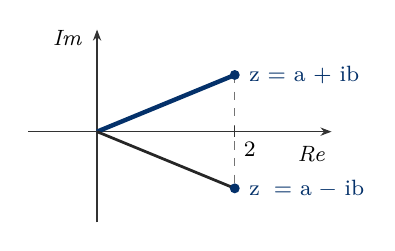
\begin{tikzpicture}[line join=round]
\draw[-{Stealth[length=4pt]},black!80] (0.720,-1.476) -- (4.572,-1.476);
\draw[-{Stealth[length=4pt]},black!80] (1.594,-2.628) -- (1.594,-0.180);
\draw[FAUblue,line width=1.6pt] (1.594,-1.476) -- (3.343,-0.756);
\draw[black!85,line width=1pt] (1.594,-1.476) -- (3.343,-2.196);
\draw[black!55,dashed] (3.343,-0.756) -- (3.343,-2.196);
\fill[FAUblue] (3.343,-0.756) circle (0.063);
\node[anchor=west,text=FAUblue,fill=white,fill opacity=0.85,text opacity=1,inner sep=1pt,font=\footnotesize] at (3.487,-0.756) {z = a + ib};
\fill[FAUblue] (3.343,-2.196) circle (0.063);
\node[anchor=west,text=FAUblue,fill=white,fill opacity=0.85,text opacity=1,inner sep=1pt,font=\footnotesize] at (3.487,-2.196) {z̅ = a \ensuremath{-} ib};
\node[anchor=east,inner sep=1pt,font=\footnotesize] at (4.536,-1.764) {\textit{Re}};
\node[anchor=east,inner sep=1pt,font=\footnotesize] at (1.450,-0.288) {\textit{Im}};
\draw[black!80] (3.343,-1.404) -- (3.343,-1.548);
\node[anchor=west,inner sep=1pt,font=\footnotesize] at (3.415,-1.692) {2};
\end{tikzpicture}\par\smallskip{\small\raggedright \textbf{Conjugate and magnitude.} The conjugate z̅ is the mirror image of z in the real axis, and both lie at the same distance |z| = \ensuremath{\sqrt{\mathrm{a}^{2}\, +\, \mathrm{b}^{2}}} from the origin.\par}\end{minipage}
\end{center}

\begin{equationcard}{Rules for conjugate and magnitude}
\[ \begin{gathered} \text{conj}({z}\, +\, {w})\, =\, {\overline{z}}\, +\, {\overline{w}} \\ \text{conj}({z}\, \cdot \, {w})\, =\, {\overline{z}}\, \cdot \, {\overline{w}} \\ \text{Re}\, {z}\, =\, \dfrac{{z}\, +\, {\overline{z}}}{2} \\ \text{Im}\, {z}\, =\, \dfrac{{z}\, -\, {\overline{z}}}{2\mathrm{i}} \\ |{z}{w}|\, =\, |{z}|\, |{w}| \\ ||{z}|\, -\, |{w}||\, \leq \, |{z}\, +\, {w}|\, \leq \, |{z}|\, +\, |{w}| \end{gathered} \]
{\small \emph{Read it as: “the conjugate of a sum is the sum of the conjugates, and likewise for products”, where conj(z) means z̅; “the magnitude of a product is the product of the magnitudes”; the last line is the triangle inequality.}\par \textit{z} = \textit{z̅} exactly when \textit{z} is real. These are the same rules the real absolute value obeys (Theorem 2.10).}
\end{equationcard}

\begin{equationcard}{Distance and circles}
\[ \begin{gathered} |{z}\, -\, {w}|\, =\, \sqrt{({a}_{1}\, -\, {a}_{2})^{2}\, +\, ({b}_{1}\, -\, {b}_{2})^{2}} \\ \{{z}\, \in \, \mathbb{C}\, :\, |{z}\, -\, {a}|\, =\, {r}\} \end{gathered} \]
{\small \emph{Read it as: “the distance between z and w is the magnitude of their difference”, and “the set of z whose distance from a is r”.}\par Here \textit{z} = \textit{a}\textsubscript{1} + i\textit{b}\textsubscript{1}, \textit{w} = \textit{a}\textsubscript{2} + i\textit{b}\textsubscript{2}. The second set is the circle with centre \textit{a} and radius \textit{r}; “\ensuremath{<} \textit{r}” gives its inside and “\ensuremath{>} \textit{r}” its outside.}
\end{equationcard}

\begin{workedbox}{Worked example \ensuremath{\cdot} a disc in the plane}
Describe the set M = \{\textit{z} \ensuremath{\in} \ensuremath{\mathbb{C}} : |\textit{z} \ensuremath{-} (1 + i)| \ensuremath{\leq} 2\}, and decide whether 3 + i and 2 + 3i belong to it.

\Needspace{6\baselineskip}
\begin{enumerate}
\item |\textit{z} \ensuremath{-} (1 + i)| is the distance from \textit{z} to the point 1 + i, so M is the closed disc with centre 1 + i and radius 2, boundary included.
\item For 3 + i: |(3 + i) \ensuremath{-} (1 + i)| = |2| = 2 \ensuremath{\leq} 2, so it lies in M, on the boundary circle.
\item For 2 + 3i: |1 + 2i| = \ensuremath{\sqrt{5}} \ensuremath{\approx} 2.24 \ensuremath{>} 2, so it lies outside M.
\end{enumerate}

Check with a sketch: 3 + i is two units right of the centre, exactly on the circle, and 2 + 3i is further out, up and to the right.
\end{workedbox}
\end{keepsection}

\begin{keepsection}
\Needspace{12\baselineskip}
\subsection{Polar and exponential form}

\begin{equationcard}{Polar form and Euler’s formula}
\[ \begin{gathered} {z}\, =\, |{z}|(\cos \, φ\, +\, \mathrm{i}\, \sin \, φ) \\ \mathrm{e}^{\mathrm{i}φ}\, =\, \cos \, φ\, +\, \mathrm{i}\, \sin \, φ \\ {z}\, =\, |{z}|\mathrm{e}^{\mathrm{i}φ} \end{gathered} \]
{\small \emph{Read it as: “z is its magnitude times cos phi plus i sin phi”, and “e to the i phi is cos phi plus i sin phi” (Euler’s formula), so “z is its magnitude times e to the i phi”.}\par φ = arg \textit{z} is the argument, the angle from the positive real axis, taken in 0 \ensuremath{\leq} φ \ensuremath{<} 2π. With \textit{r} = |\textit{z}|: \textit{a} = \textit{r} cos φ and \textit{b} = \textit{r} sin φ. Find φ from tan φ = {\small\ensuremath{\dfrac{{b}}{{a}}}} using the quadrant of (\textit{a}, \textit{b}), exactly as for polar coordinates in §3.6. For \textit{z} = 0 the angle is undefined.}
\end{equationcard}

\Needspace{14\baselineskip}
\begin{center}
\begin{minipage}[t]{0.950\linewidth}\centering
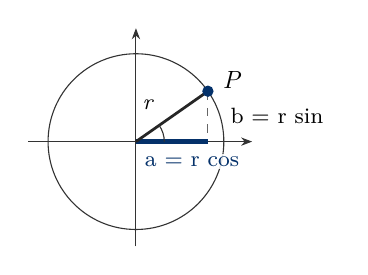
\begin{tikzpicture}[line join=round]
\draw[-{Stealth[length=4pt]},black!80] (0.144,-1.512) -- (2.988,-1.512);
\draw[-{Stealth[length=4pt]},black!80] (1.512,-2.844) -- (1.512,-0.072);
\draw[black!80] (1.512,-1.512) circle (1.116);
\draw[black!60,dashed] (2.426,-0.872) -- (2.426,-1.512);
\draw[FAUblue,line width=2pt] (1.512,-1.512) -- (2.426,-1.512);
\draw[black!85,line width=1pt] (1.512,-1.512) -- (2.426,-0.872);
\draw[black!80] (1.872,-1.512) arc (0:35.0:0.360);
\fill[FAUblue] (2.426,-0.872) circle (0.072);
\node[,inner sep=1pt,font=\footnotesize] at (2.101,-1.396) {\textit{φ}};
\node[anchor=west,text=FAUblue,fill=white,fill opacity=0.85,text opacity=1,inner sep=1pt,font=\footnotesize] at (1.584,-1.764) {a = r cos φ};
\node[anchor=west,inner sep=1pt,font=\footnotesize] at (2.671,-1.192) {b = r sin φ};
\node[anchor=east,inner sep=1pt,font=\footnotesize] at (1.789,-1.048) {\textit{r}};
\node[anchor=west,inner sep=1pt,font=\small] at (2.570,-0.728) {\textit{P}};
\end{tikzpicture}\par\smallskip{\small\raggedright \textbf{Polar form.} The number at length \textit{r} = |\textit{z}| and angle φ has real part \textit{r} cos φ and imaginary part \textit{r} sin φ.\par}\end{minipage}
\end{center}

\begin{equationcard}{Rules for e\textsuperscript{iφ}}
\[ \begin{gathered} \mathrm{e}^{\mathrm{i}(φ_{1}\, +\, φ_{2})}\, =\, \mathrm{e}^{\mathrm{i}φ_{1}}\mathrm{e}^{\mathrm{i}φ_{2}} \\ (\mathrm{e}^{\mathrm{i}φ})^{{n}}\, =\, \mathrm{e}^{\mathrm{i}{n}φ} \\ |\mathrm{e}^{\mathrm{i}φ}|\, =\, 1 \\ \mathrm{e}^{\mathrm{i}(φ\, +\, 2{k}π)}\, =\, \mathrm{e}^{\mathrm{i}φ} \end{gathered} \]
{\small \emph{Read it as: “adding angles multiplies the exponentials”, and “e to the i phi always lies on the unit circle”.}\par Here \textit{k} \ensuremath{\in} \ensuremath{\mathbb{Z}}. In the notes Euler’s formula is at first an abbreviation; it is proved properly later with Taylor series. It gives \textit{z̅} = |\textit{z}|e\textsuperscript{\ensuremath{-}iφ}, and \textit{z} = \textit{w} exactly when |\textit{z}| = |\textit{w}| and the arguments differ by a multiple of 2π.}
\end{equationcard}

\begin{workedbox}{Worked example \ensuremath{\cdot} normal form to exponential form}
Write \textit{z} = \ensuremath{-}\ensuremath{\sqrt{3}} + i in exponential form.

\Needspace{8\baselineskip}
\begin{enumerate}
\item The magnitude is |\textit{z}| = \ensuremath{\sqrt{3\, +\, 1}} = \ensuremath{\sqrt{4}} = 2.
\item The real part is negative and the imaginary part positive, so \textit{z} lies in quadrant II and the arctan value must be shifted by π.
\item arctan({\small\ensuremath{\dfrac{1}{-\sqrt{3}}}}) = \ensuremath{-}{\small\ensuremath{\dfrac{π}{6}}}, so φ = \ensuremath{-}{\small\ensuremath{\dfrac{π}{6}}} + π = {\small\ensuremath{\dfrac{5π}{6}}}.
\item Therefore \textit{z} = 2e\textsuperscript{i5π/6}.
\end{enumerate}

Check: 2 cos({\small\ensuremath{\dfrac{5π}{6}}}) = \ensuremath{-}\ensuremath{\sqrt{3}} and 2 sin({\small\ensuremath{\dfrac{5π}{6}}}) = 1, which recovers \ensuremath{-}\ensuremath{\sqrt{3}} + i.
\end{workedbox}
\end{keepsection}

\begin{keepsection}
\Needspace{11\baselineskip}
\subsection{Multiplying and dividing in polar form}

\begin{equationcard}{Product and quotient}
\[ \begin{gathered} {z}{w}\, =\, |{z}|\, |{w}|\, \mathrm{e}^{\mathrm{i}(φ\, +\, ψ)} \\ \dfrac{{z}}{{w}}\, =\, \dfrac{|{z}|}{|{w}|}\, \mathrm{e}^{\mathrm{i}(φ\, -\, ψ)} \end{gathered} \]
{\small \emph{Read it as: “to multiply, multiply the lengths and add the angles; to divide, divide the lengths and subtract the angles”.}\par Here \textit{z} = |\textit{z}|e\textsuperscript{iφ}, \textit{w} = |\textit{w}|e\textsuperscript{iψ} and \textit{w} \ensuremath{\neq} 0. This follows from the addition theorems for sine and cosine (§3.5). Geometrically, multiplying by \textit{w} turns by ψ and stretches by |\textit{w}|.}
\end{equationcard}

\begin{workedbox}{Worked example \ensuremath{\cdot} multiply and divide in polar form}
Let \textit{z} = 2e\textsuperscript{iπ/3} and \textit{w} = 4e\textsuperscript{iπ/6}.

\Needspace{4\baselineskip}
\begin{enumerate}
\item Product: lengths 2 \ensuremath{\cdot} 4 = 8, angles {\small\ensuremath{\dfrac{π}{3}}} + {\small\ensuremath{\dfrac{π}{6}}} = {\small\ensuremath{\dfrac{π}{2}}}, so \textit{z}\textit{w} = 8e\textsuperscript{iπ/2} = 8i.
\item Quotient: lengths {\small\ensuremath{\dfrac{2}{4}}} = {\small\ensuremath{\dfrac{1}{2}}}, angles {\small\ensuremath{\dfrac{π}{3}}} \ensuremath{-} {\small\ensuremath{\dfrac{π}{6}}} = {\small\ensuremath{\dfrac{π}{6}}}, so {\small\ensuremath{\dfrac{{z}}{{w}}}} = {\small\ensuremath{\dfrac{1}{2}}}e\textsuperscript{iπ/6} = {\small\ensuremath{\dfrac{1}{2}}}({\small\ensuremath{\dfrac{\sqrt{3}}{2}}} + {\small\ensuremath{\dfrac{1}{2}}}i) = {\small\ensuremath{\dfrac{\sqrt{3}}{4}}} + {\small\ensuremath{\dfrac{1}{4}}}i.
\end{enumerate}

Check the product in normal form: \textit{z} = 1 + i\ensuremath{\sqrt{3}} and \textit{w} = 2\ensuremath{\sqrt{3}} + 2i, and (1 + i\ensuremath{\sqrt{3}})(2\ensuremath{\sqrt{3}} + 2i) = 2\ensuremath{\sqrt{3}} + 2i + 6i \ensuremath{-} 2\ensuremath{\sqrt{3}} = 8i.
\end{workedbox}

\Needspace{6\baselineskip}
\begin{notebox}\textbf{Trap:} |\textit{z}|\textsuperscript{2} is not \textit{z}\textsuperscript{2} for complex numbers. For \textit{z} = 1 + i, |\textit{z}|\textsuperscript{2} = (1 + i)(1 \ensuremath{-} i) = 2, but (1 + i)\textsuperscript{2} = 2i. Only for real numbers do the two agree.\end{notebox}

\Needspace{6\baselineskip}
\begin{notebox}\textbf{Sign check:} arctan({\small\ensuremath{\dfrac{{b}}{{a}}}}) only returns angles between \ensuremath{-}{\small\ensuremath{\dfrac{π}{2}}} and {\small\ensuremath{\dfrac{π}{2}}}. Decide the quadrant from the signs of \textit{a} and \textit{b} first, then add π (quadrants II and III) or 2π (quadrant IV) to land in [0, 2π).\end{notebox}

\Needspace{6\baselineskip}
\begin{notebox}\textbf{Memory hook:} normal form for adding, polar form for multiplying. Each form makes one operation easy and the other awkward.\end{notebox}

\Needspace{11\baselineskip}
\begin{notebox}\textbf{Near miss:} for \textit{z} = \ensuremath{-}1 \ensuremath{-} i, tan φ = {\small\ensuremath{\dfrac{-1}{-1}}} = 1 suggests φ = {\small\ensuremath{\dfrac{π}{4}}}, but that angle points into quadrant I. Both parts are negative, so add π: φ = {\small\ensuremath{\dfrac{5π}{4}}} and \textit{z} = \ensuremath{\sqrt{2}}e\textsuperscript{i5π/4}.\end{notebox}

\begin{recallbox}{Recall check \ensuremath{\cdot} answer before opening}
\Needspace{5\baselineskip}
\begin{enumerate}
\item What is (2 + i)(2 \ensuremath{-} i), and why is it real?
\item What happens to lengths and angles when you divide two complex numbers?
\item What is {\small\ensuremath{\dfrac{1}{\mathrm{i}}}} in normal form?
\end{enumerate}

\nopagebreak[4]{\small\itshape Answers: see “4.1 Definitions and Basic Arithmetic Operations” under Answers at the end.}
\end{recallbox}
\end{keepsection}
\end{keepsection}

\begin{keepsection}
\Needspace{12\baselineskip}
\section{4.2 Roots and Powers}

\Needspace{9\baselineskip}
Polar multiplication from §4.1 turns a power into one stretch and one turn. Run backwards, it solves \textit{w}\textsuperscript{\textit{n}} = \textit{z}, which always has exactly \textit{n} answers in \ensuremath{\mathbb{C}}.

\begin{plainbox}\textbf{In plain words:} raising a number to the power k stretches its length to the k-th power and turns its angle k times over; this is \textbf{de Moivre’s formula}. An \textbf{n-th root} undoes that: take the ordinary root of the length and divide the angle by n. Because an angle is only known up to whole turns, dividing gives n different answers, spread evenly round a circle like the corners of a regular polygon.\end{plainbox}

\begin{keepsection}
\Needspace{10\baselineskip}
\subsection{Powers}

\begin{equationcard}{De Moivre’s formula}
\[ \begin{gathered} {z}^{{k}}\, =\, |{z}|^{{k}}(\cos ({k}φ)\, +\, \mathrm{i}\, \sin ({k}φ))\, =\, |{z}|^{{k}}\mathrm{e}^{\mathrm{i}{k}φ} \end{gathered} \]
{\small \emph{Read it as: “z to the k is the magnitude to the k times e to the i k phi”.}\par Here \textit{z} = |\textit{z}|e\textsuperscript{iφ} and \textit{k} \ensuremath{\in} \ensuremath{\mathbb{N}}. It is polar multiplication of \textit{z} by itself \textit{k} times. Reduce \textit{k}φ by multiples of 2π to bring it back into [0, 2π).}
\end{equationcard}

\begin{workedbox}{Worked example \ensuremath{\cdot} a sixth power}
Compute (1 \ensuremath{-} i)\textsuperscript{6}.

\Needspace{5\baselineskip}
\begin{enumerate}
\item Polar form: |1 \ensuremath{-} i| = \ensuremath{\sqrt{2}}, and the point is in quadrant IV, so φ = {\small\ensuremath{\dfrac{7π}{4}}} and 1 \ensuremath{-} i = \ensuremath{\sqrt{2}}e\textsuperscript{i7π/4}.
\item De Moivre: the length becomes (\ensuremath{\sqrt{2}})\textsuperscript{6} = 8 and the angle 6 \ensuremath{\cdot} {\small\ensuremath{\dfrac{7π}{4}}} = {\small\ensuremath{\dfrac{21π}{2}}}.
\item Reduce the angle: {\small\ensuremath{\dfrac{21π}{2}}} = 10π + {\small\ensuremath{\dfrac{π}{2}}}, so the angle is {\small\ensuremath{\dfrac{π}{2}}} and (1 \ensuremath{-} i)\textsuperscript{6} = 8e\textsuperscript{iπ/2} = 8i.
\end{enumerate}

Check by squaring in normal form: (1 \ensuremath{-} i)\textsuperscript{2} = \ensuremath{-}2i, and (\ensuremath{-}2i)\textsuperscript{3} = \ensuremath{-}8i\textsuperscript{3} = 8i.
\end{workedbox}
\end{keepsection}

\begin{keepsection}
\Needspace{11\baselineskip}
\subsection{n-th roots}

\begin{equationcard}{The n roots of a complex number}
\[ \begin{gathered} {w}^{{n}}\, =\, {z} \\ {w}_{{k}}\, =\, |{z}|^{1/{n}}\, \mathrm{e}^{\mathrm{i}(φ\, +\, 2{k}π)/{n}},\, {k}\, =\, 0,\, 1,\, …,\, {n}\, -\, 1 \end{gathered} \]
{\small \emph{Read it as: “the k-th root w k is the real n-th root of the magnitude times e to the i, phi plus 2 k pi, over n”.}\par Here \textit{z} = |\textit{z}|e\textsuperscript{iφ} \ensuremath{\neq} 0 and \textit{n} \ensuremath{\in} \ensuremath{\mathbb{N}}; |\textit{z}|\textsuperscript{1/\textit{n}} is the ordinary non-negative real root. There are exactly \textit{n} distinct roots. They are the corners of a regular \textit{n}-gon on the circle of radius |\textit{z}|\textsuperscript{1/\textit{n}}, neighbours {\small\ensuremath{\dfrac{2π}{{n}}}} apart, the first at angle {\small\ensuremath{\dfrac{φ}{{n}}}}.}
\end{equationcard}

\Needspace{14\baselineskip}
\begin{center}
\begin{minipage}[t]{0.950\linewidth}\centering
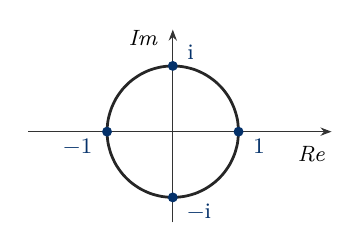
\begin{tikzpicture}[line join=round]
\draw[-{Stealth[length=4pt]},black!80] (0.720,-1.476) -- (4.572,-1.476);
\draw[-{Stealth[length=4pt]},black!80] (2.556,-2.628) -- (2.556,-0.180);
\draw[black!85,line width=1pt] plot[smooth,tension=0.5] coordinates {(3.391,-1.476) (3.378,-1.331) (3.340,-1.191) (3.279,-1.059) (3.195,-0.939) (3.093,-0.837) (2.973,-0.753) (2.841,-0.691) (2.701,-0.654) (2.556,-0.641) (2.411,-0.654) (2.271,-0.691) (2.139,-0.753) (2.019,-0.837) (1.917,-0.939) (1.833,-1.059) (1.772,-1.191) (1.734,-1.331) (1.721,-1.476) (1.734,-1.621) (1.772,-1.761) (1.833,-1.893) (1.917,-2.013) (2.019,-2.115) (2.139,-2.199) (2.271,-2.261) (2.411,-2.298) (2.556,-2.311) (2.701,-2.298) (2.841,-2.261) (2.973,-2.199) (3.093,-2.115) (3.195,-2.013) (3.279,-1.893) (3.340,-1.761) (3.378,-1.621) (3.391,-1.476)};
\fill[FAUblue] (3.391,-1.476) circle (0.063);
\node[anchor=west,text=FAUblue,fill=white,fill opacity=0.85,text opacity=1,inner sep=1pt,font=\footnotesize] at (3.535,-1.656) {1};
\fill[FAUblue] (2.556,-0.641) circle (0.063);
\node[anchor=west,text=FAUblue,fill=white,fill opacity=0.85,text opacity=1,inner sep=1pt,font=\footnotesize] at (2.700,-0.461) {i};
\fill[FAUblue] (1.721,-1.476) circle (0.063);
\node[anchor=east,text=FAUblue,fill=white,fill opacity=0.85,text opacity=1,inner sep=1pt,font=\footnotesize] at (1.577,-1.656) {\ensuremath{-}1};
\fill[FAUblue] (2.556,-2.311) circle (0.063);
\node[anchor=west,text=FAUblue,fill=white,fill opacity=0.85,text opacity=1,inner sep=1pt,font=\footnotesize] at (2.700,-2.491) {\ensuremath{-}i};
\node[anchor=east,inner sep=1pt,font=\footnotesize] at (4.536,-1.764) {\textit{Re}};
\node[anchor=east,inner sep=1pt,font=\footnotesize] at (2.412,-0.288) {\textit{Im}};
\end{tikzpicture}\par\smallskip{\small\raggedright \textbf{The fourth roots of 1.} The four solutions of \textit{w}\textsuperscript{4} = 1 are 1, i, \ensuremath{-}1 and \ensuremath{-}i: the corners of a square on the unit circle, a quarter turn apart.\par}\end{minipage}
\end{center}

\Needspace{8\baselineskip}
Why the formula: write \textit{w} = |\textit{w}|e\textsuperscript{iψ}. Then \textit{w}\textsuperscript{\textit{n}} = |\textit{w}|\textsuperscript{\textit{n}}e\textsuperscript{i\textit{n}ψ}, and this equals |\textit{z}|e\textsuperscript{iφ} exactly when

\Needspace{6\baselineskip}
\begin{enumerate}
\item |\textit{w}|\textsuperscript{\textit{n}} = |\textit{z}|, so |\textit{w}| = |\textit{z}|\textsuperscript{1/\textit{n}}, and
\item \textit{n}ψ = φ + 2\textit{k}π for some \textit{k} \ensuremath{\in} \ensuremath{\mathbb{Z}}, so ψ = {\small\ensuremath{\dfrac{φ\, +\, 2{k}π}{{n}}}}.
\item \textit{k} = \textit{n} gives the angle of \textit{k} = 0 plus a full turn, so only \textit{k} = 0, …, \textit{n} \ensuremath{-} 1 give different numbers.
\end{enumerate}

\begin{equationcard}{Rules for roots}
\[ \begin{gathered} {z}^{1/{n}}\, \cdot \, {w}^{1/{n}}\, =\, ({z}\, \cdot \, {w})^{1/{n}} \\ \dfrac{{z}^{1/{n}}}{{w}^{1/{n}}}\, =\, \left(\dfrac{{z}}{{w}}\right)^{1/{n}} \end{gathered} \]
{\small \emph{Read it as: “the product of n-th roots is an n-th root of the product”.}\par For \textit{w} \ensuremath{\neq} 0 in the quotient. Because each root has \textit{n} values, these hold only for suitably chosen values, not for any choice.}
\end{equationcard}

\begin{workedbox}{Worked example \ensuremath{\cdot} the cube roots of \ensuremath{-}8}
Solve \textit{w}\textsuperscript{3} = \ensuremath{-}8.

\Needspace{7\baselineskip}
\begin{enumerate}
\item Polar form of the right side: \ensuremath{-}8 = 8e\textsuperscript{iπ}, so |\textit{z}| = 8 and φ = π.
\item Length of every root: 8\textsuperscript{1/3} = 2.
\item Angles: {\small\ensuremath{\dfrac{π\, +\, 2{k}π}{3}}} for \textit{k} = 0, 1, 2, that is {\small\ensuremath{\dfrac{π}{3}}}, π and {\small\ensuremath{\dfrac{5π}{3}}}.
\item The roots are \textit{w}\textsubscript{0} = 2e\textsuperscript{iπ/3} = 1 + i\ensuremath{\sqrt{3}}, \textit{w}\textsubscript{1} = 2e\textsuperscript{iπ} = \ensuremath{-}2 and \textit{w}\textsubscript{2} = 2e\textsuperscript{i5π/3} = 1 \ensuremath{-} i\ensuremath{\sqrt{3}}.
\end{enumerate}

Check: (\ensuremath{-}2)\textsuperscript{3} = \ensuremath{-}8, and by de Moivre (2e\textsuperscript{iπ/3})\textsuperscript{3} = 8e\textsuperscript{iπ} = \ensuremath{-}8. The three roots also sum to 0, as the corners of an equilateral triangle centred at the origin must.
\end{workedbox}
\end{keepsection}

\begin{keepsection}
\Needspace{15\baselineskip}
\subsection{Application: phasors in AC circuits}

\Needspace{12\baselineskip}
An alternating voltage \textit{U}(\textit{t}) = \textit{U}\textsubscript{0} sin(ω\textit{t}) is replaced by the rotating complex voltage \textit{U}(\textit{t}) = \textit{U}\textsubscript{0}e\textsuperscript{iω\textit{t}}; the real signal is recovered as its imaginary part. A phase shift then becomes a fixed angle between rotating arrows, and derivatives become multiplication by iω.

\begin{equationcard}{Current through a coil}
\[ \begin{gathered} \dfrac{{U}}{{L}}\, =\, \dfrac{\mathrm{d}}{\mathrm{d}{t}}\, {I} \\ {I}\, =\, \dfrac{{U}}{\mathrm{i}ω{L}}\, =\, \dfrac{{U}_{0}}{ω{L}}\, \mathrm{e}^{\mathrm{i}(ω{t}\, -\, π/2)} \end{gathered} \]
{\small \emph{Read it as: “the voltage over L is the rate of change of current”, so “the current phasor is the voltage phasor divided by i omega L”.}\par \textit{L} in H, ω in s\textsuperscript{\ensuremath{-}1}, \textit{U}\textsubscript{0} in V, so \textit{I}\textsubscript{0} = {\small\ensuremath{\dfrac{{U}_{0}}{ω{L}}}} is in A. Since {\small\ensuremath{\dfrac{1}{\mathrm{i}}}} = \ensuremath{-}i = e\textsuperscript{\ensuremath{-}iπ/2}, the current lags the voltage by {\small\ensuremath{\dfrac{π}{2}}}. (The notes write Û and Î for the amplitudes \textit{U}\textsubscript{0}, \textit{I}\textsubscript{0}, and w for ω.)}
\end{equationcard}

\begin{workedbox}{Worked example \ensuremath{\cdot} amplitude and phase of a coil current}
A coil with \textit{L} = 0.2 H is driven by \textit{U}(\textit{t}) = 10 V \ensuremath{\cdot} sin(50 s\textsuperscript{\ensuremath{-}1} \ensuremath{\cdot} \textit{t}).

\Needspace{4\baselineskip}
\begin{enumerate}
\item Amplitude: \textit{I}\textsubscript{0} = {\small\ensuremath{\dfrac{{U}_{0}}{ω{L}}}} = {\small\ensuremath{\dfrac{10\, \mathrm{V}}{50\, \mathrm{s}^{-1}\, \cdot \, 0.2\, \mathrm{H}}}} = 1 A.
\item Phase: the factor {\small\ensuremath{\dfrac{1}{\mathrm{i}}}} = e\textsuperscript{\ensuremath{-}iπ/2} shifts the current by \ensuremath{-}{\small\ensuremath{\dfrac{π}{2}}}, so \textit{I}(\textit{t}) = 1 A \ensuremath{\cdot} sin(50 s\textsuperscript{\ensuremath{-}1} \ensuremath{\cdot} \textit{t} \ensuremath{-} {\small\ensuremath{\dfrac{π}{2}}}).
\end{enumerate}

Check the units: V divided by s\textsuperscript{\ensuremath{-}1} \ensuremath{\cdot} H is V divided by Ω, which is A, since 1 H \ensuremath{\cdot} s\textsuperscript{\ensuremath{-}1} = 1 Ω.
\end{workedbox}

\Needspace{6\baselineskip}
\begin{notebox}\textbf{Trap:} the n-th root of a complex number is not one number. Writing “\ensuremath{\sqrt{-1}} = i” picks one of two square roots of \ensuremath{-}1; the other is \ensuremath{-}i.\end{notebox}

\Needspace{6\baselineskip}
\begin{notebox}\textbf{Sign check:} multiplying by i turns counterclockwise by {\small\ensuremath{\dfrac{π}{2}}}; dividing by i turns clockwise by {\small\ensuremath{\dfrac{π}{2}}}. That is why a coil’s current lags its voltage.\end{notebox}

\Needspace{7\baselineskip}
\begin{notebox}\textbf{Memory hook:} for \textit{n} \ensuremath{\geq} 2 the \textit{n} roots balance around the origin, so they add up to 0. If yours do not, an angle is wrong.\end{notebox}

\Needspace{10\baselineskip}
\begin{notebox}\textbf{Near miss:} “\ensuremath{\sqrt{{z}}} \ensuremath{\cdot} \ensuremath{\sqrt{{w}}} = \ensuremath{\sqrt{{z}{w}}}” with \textit{z} = \textit{w} = \ensuremath{-}1 and the value i for each root gives i \ensuremath{\cdot} i = \ensuremath{-}1, but \ensuremath{\sqrt{1}} = 1 for the value 1. The rule needs suitably chosen values: taking \ensuremath{-}1 as the value of \ensuremath{\sqrt{1}} makes it hold.\end{notebox}

\begin{recallbox}{Recall check \ensuremath{\cdot} answer before opening}
\Needspace{4\baselineskip}
\begin{enumerate}
\item How many distinct fifth roots does i have?
\item What angle separates neighbouring solutions of \textit{w}\textsuperscript{6} = \textit{z}?
\end{enumerate}

\nopagebreak[4]{\small\itshape Answers: see “4.2 Roots and Powers” under Answers at the end.}
\end{recallbox}
\end{keepsection}
\end{keepsection}

\begin{keepsection}
\Needspace{13\baselineskip}
\section{4.3 Special Complex Functions}

\Needspace{10\baselineskip}
With complex numbers available, polynomials always split into linear factors, and the exponential, logarithm, sine and cosine extend to complex inputs. The extensions keep the familiar rules but gain new behaviour: the exponential repeats, and the logarithm has to choose an angle.

\begin{plainbox}\textbf{In plain words:} over the complex numbers, a polynomial of degree n always has n zeros, counted with repeats; this is the \textbf{fundamental theorem of algebra}. The \textbf{complex exponential} e to the x + iy stretches by e to the x and turns by y; since a full turn changes nothing, it repeats when you add 2πi. To undo it, the \textbf{complex logarithm} must pick one angle from each family, and the notes take the angle in [0, 2π). \textbf{Complex sine} and \textbf{cosine} are built from exponentials.\end{plainbox}

\begin{keepsection}
\Needspace{11\baselineskip}
\subsection{Polynomials}

\begin{equationcard}{Fundamental theorem of algebra}
\[ \begin{gathered} {P}({z})\, =\, {a}_{{n}}{z}^{{n}}\, +\, …\, +\, {a}_{1}{z}\, +\, {a}_{0} \\ {P}({z})\, =\, {a}_{{n}}({z}\, -\, {z}_{1})({z}\, -\, {z}_{2})\, …\, ({z}\, -\, {z}_{{n}}) \end{gathered} \]
{\small \emph{Read it as: “a complex polynomial of degree n factors completely into n linear factors”.}\par Coefficients \textit{a}\textsubscript{0}, …, \textit{a}\textsubscript{\textit{n}} \ensuremath{\in} \ensuremath{\mathbb{C}} with \textit{a}\textsubscript{\textit{n}} \ensuremath{\neq} 0, and \textit{n} \ensuremath{\in} \ensuremath{\mathbb{N}}. The zeros \textit{z}\textsubscript{1}, …, \textit{z}\textsubscript{\textit{n}} need not be distinct; grouping equal ones gives \textit{a}\textsubscript{\textit{n}}(\textit{z} \ensuremath{-} \textit{z}\textsubscript{1})\textsuperscript{\textit{m}\textsubscript{1}} … (\textit{z} \ensuremath{-} \textit{z}\textsubscript{\textit{l}})\textsuperscript{\textit{m}\textsubscript{\textit{l}}}, where the multiplicities add up to \textit{n}. The notes state this without proof.}
\end{equationcard}

\begin{equationcard}{Real coefficients}
\[ \begin{gathered} {P}({z}_{0})\, =\, 0\, \Rightarrow \, {P}({\overline{z}}_{0})\, =\, 0 \\ ({z}\, -\, {z}_{0})({z}\, -\, {\overline{z}}_{0})\, =\, {z}^{2}\, -\, 2\, \text{Re}({z}_{0})\, {z}\, +\, |{z}_{0}|^{2} \end{gathered} \]
{\small \emph{Read it as: “if z nought is a zero, so is its conjugate”, and “the pair multiplies to a quadratic with real coefficients”.}\par Holds when every coefficient is real. Consequences: non-real zeros come in conjugate pairs; a polynomial of odd degree has at least one real zero; and the polynomial factors into real linear and real quadratic factors.}
\end{equationcard}

\Needspace{14\baselineskip}
\begin{center}
\begin{minipage}[t]{0.950\linewidth}\centering
\begin{tikzpicture}[line join=round]
\draw[-{Stealth[length=4pt]},black!80] (0.720,-1.476) -- (4.572,-1.476);
\draw[-{Stealth[length=4pt]},black!80] (1.944,-2.628) -- (1.944,-0.180);
\draw[black!55,dashed] (1.944,-0.590) -- (1.944,-2.362);
\fill[FAUblue] (2.964,-1.476) circle (0.063);
\node[anchor=west,text=FAUblue,fill=white,fill opacity=0.85,text opacity=1,inner sep=1pt,font=\footnotesize] at (3.108,-1.296) {1};
\fill[FAUblue] (1.944,-0.590) circle (0.063);
\node[anchor=west,text=FAUblue,fill=white,fill opacity=0.85,text opacity=1,inner sep=1pt,font=\footnotesize] at (2.088,-0.590) {2i};
\fill[FAUblue] (1.944,-2.362) circle (0.063);
\node[anchor=west,text=FAUblue,fill=white,fill opacity=0.85,text opacity=1,inner sep=1pt,font=\footnotesize] at (2.088,-2.362) {\ensuremath{-}2i};
\node[anchor=east,inner sep=1pt,font=\footnotesize] at (4.536,-1.764) {\textit{Re}};
\node[anchor=east,inner sep=1pt,font=\footnotesize] at (1.800,-0.288) {\textit{Im}};
\draw[black!80] (2.964,-1.404) -- (2.964,-1.548);
\node[,inner sep=1pt,font=\footnotesize] at (2.964,-1.764) {1};
\end{tikzpicture}\par\smallskip{\small\raggedright \textbf{Zeros of a real polynomial.} The zeros of \textit{z}\textsuperscript{3} \ensuremath{-} \textit{z}\textsuperscript{2} + 4\textit{z} \ensuremath{-} 4 are 1, 2i and \ensuremath{-}2i. The non-real pair is mirrored in the real axis, as real coefficients force.\par}\end{minipage}
\end{center}

\begin{workedbox}{Worked example \ensuremath{\cdot} factor over \ensuremath{\mathbb{C}} and over \ensuremath{\mathbb{R}}}
Find all zeros of \textit{P}(\textit{z}) = \textit{z}\textsuperscript{3} \ensuremath{-} \textit{z}\textsuperscript{2} + 4\textit{z} \ensuremath{-} 4 and factor it both ways.

\Needspace{5\baselineskip}
\begin{enumerate}
\item Group the terms: \textit{z}\textsuperscript{2}(\textit{z} \ensuremath{-} 1) + 4(\textit{z} \ensuremath{-} 1) = (\textit{z} \ensuremath{-} 1)(\textit{z}\textsuperscript{2} + 4).
\item \textit{z}\textsuperscript{2} + 4 = 0 gives \textit{z}\textsuperscript{2} = \ensuremath{-}4 = 4e\textsuperscript{iπ}, whose two square roots are 2e\textsuperscript{iπ/2} = 2i and 2e\textsuperscript{i3π/2} = \ensuremath{-}2i.
\item Over \ensuremath{\mathbb{C}}: \textit{P}(\textit{z}) = (\textit{z} \ensuremath{-} 1)(\textit{z} \ensuremath{-} 2i)(\textit{z} + 2i). Over \ensuremath{\mathbb{R}}: \textit{P}(\textit{z}) = (\textit{z} \ensuremath{-} 1)(\textit{z}\textsuperscript{2} + 4).
\end{enumerate}

Check with the pair formula: for \textit{z}\textsubscript{0} = 2i, \ensuremath{-}2 Re(2i) = 0 and |2i|\textsuperscript{2} = 4, giving \textit{z}\textsuperscript{2} + 4. Degree 3 and three zeros, one of them real, as odd degree requires.
\end{workedbox}
\end{keepsection}

\begin{keepsection}
\Needspace{11\baselineskip}
\subsection{The complex exponential}

\begin{equationcard}{Complex exponential function}
\[ \begin{gathered} \mathrm{e}^{{z}}\, =\, \mathrm{e}^{{x}\, +\, \mathrm{i}{y}}\, =\, \mathrm{e}^{{x}}(\cos \, {y}\, +\, \mathrm{i}\, \sin \, {y}) \\ |\mathrm{e}^{{z}}|\, =\, \mathrm{e}^{{x}} \\ \mathrm{e}^{{z}\, +\, 2{k}π\mathrm{i}}\, =\, \mathrm{e}^{{z}} \\ \mathrm{e}^{{z}\, +\, {w}}\, =\, \mathrm{e}^{{z}}\mathrm{e}^{{w}} \end{gathered} \]
{\small \emph{Read it as: “e to the x plus i y is e to the x times cos y plus i sin y”: the real part sets the length, the imaginary part the angle.}\par Defined for every \textit{z} \ensuremath{\in} \ensuremath{\mathbb{C}}. Unlike the real exponential it is periodic, with period 2πi (\textit{k} \ensuremath{\in} \ensuremath{\mathbb{Z}}). It is never 0, because its length e\textsuperscript{\textit{x}} is positive.}
\end{equationcard}

\begin{workedbox}{Worked example \ensuremath{\cdot} evaluate an exponential}
Compute e\textsuperscript{2 + iπ/3} in normal form and give its magnitude.

\Needspace{5\baselineskip}
\begin{enumerate}
\item Split the exponent: real part 2, imaginary part {\small\ensuremath{\dfrac{π}{3}}}.
\item e\textsuperscript{2 + iπ/3} = e\textsuperscript{2}(cos {\small\ensuremath{\dfrac{π}{3}}} + i sin {\small\ensuremath{\dfrac{π}{3}}}) = e\textsuperscript{2}({\small\ensuremath{\dfrac{1}{2}}} + i{\small\ensuremath{\dfrac{\sqrt{3}}{2}}}).
\item With e\textsuperscript{2} \ensuremath{\approx} 7.389: e\textsuperscript{2 + iπ/3} \ensuremath{\approx} 3.69 + 6.40i, and |e\textsuperscript{2 + iπ/3}| = e\textsuperscript{2} \ensuremath{\approx} 7.39.
\end{enumerate}

Check: \ensuremath{\sqrt{3.69^{2}\, +\, 6.40^{2}}} \ensuremath{\approx} \ensuremath{\sqrt{54.6}} \ensuremath{\approx} 7.39, the same length.
\end{workedbox}
\end{keepsection}

\begin{keepsection}
\Needspace{11\baselineskip}
\subsection{The complex logarithm}

\begin{equationcard}{Complex logarithm}
\[ \begin{gathered} \ln \, {z}\, =\, \ln |{z}|\, +\, \mathrm{i}φ \\ \mathrm{e}^{\ln \, {z}}\, =\, {z} \end{gathered} \]
{\small \emph{Read it as: “ln z is the real log of the magnitude plus i times the angle”.}\par For \textit{z} = |\textit{z}|e\textsuperscript{iφ} \ensuremath{\neq} 0 with 0 \ensuremath{\leq} φ \ensuremath{<} 2π, so the domain is \ensuremath{\mathbb{C}}\textbackslash{}\{0\}, and every value lies in the strip 0 \ensuremath{\leq} Im \ensuremath{<} 2π. Without fixing the angle range, ln \textit{z} would be defined only up to adding 2\textit{k}πi. Negative real numbers now have logarithms: ln(\ensuremath{-}1) = iπ.}
\end{equationcard}

\begin{workedbox}{Worked example \ensuremath{\cdot} two logarithms}
Find ln(\ensuremath{-}e) and ln(1 + i).

\Needspace{4\baselineskip}
\begin{enumerate}
\item \ensuremath{-}e = e \ensuremath{\cdot} e\textsuperscript{iπ}, so ln(\ensuremath{-}e) = ln e + iπ = 1 + iπ.
\item 1 + i = \ensuremath{\sqrt{2}}e\textsuperscript{iπ/4}, so ln(1 + i) = ln \ensuremath{\sqrt{2}} + i{\small\ensuremath{\dfrac{π}{4}}} = {\small\ensuremath{\dfrac{1}{2}}} ln 2 + i{\small\ensuremath{\dfrac{π}{4}}} \ensuremath{\approx} 0.347 + 0.785i.
\end{enumerate}

Check the second: e\textsuperscript{ln(1 + i)} = e\textsuperscript{(ln 2)/2}e\textsuperscript{iπ/4} = \ensuremath{\sqrt{2}}({\small\ensuremath{\dfrac{\sqrt{2}}{2}}} + i{\small\ensuremath{\dfrac{\sqrt{2}}{2}}}) = 1 + i.
\end{workedbox}
\end{keepsection}

\begin{keepsection}
\Needspace{12\baselineskip}
\subsection{Complex sine and cosine}

\begin{equationcard}{Sine and cosine of a complex number}
\[ \begin{gathered} \sin \, {z}\, =\, \dfrac{\mathrm{e}^{\mathrm{i}{z}}\, -\, \mathrm{e}^{-\mathrm{i}{z}}}{2\mathrm{i}} \\ \cos \, {z}\, =\, \dfrac{\mathrm{e}^{\mathrm{i}{z}}\, +\, \mathrm{e}^{-\mathrm{i}{z}}}{2} \end{gathered} \]
{\small \emph{Read it as: “sine z is e to the i z minus e to the minus i z, over 2 i”, and likewise for cosine with a plus over 2.}\par For real \textit{x} these follow from adding and subtracting e\textsuperscript{i\textit{x}} = cos \textit{x} + i sin \textit{x} and e\textsuperscript{\ensuremath{-}i\textit{x}} = cos \textit{x} \ensuremath{-} i sin \textit{x}; for complex \textit{z} they are the definition. They keep period 2π, sin\textsuperscript{2} \textit{z} + cos\textsuperscript{2} \textit{z} = 1 and the addition theorems, and their zeros are only the real ones: sin \textit{z} = 0 \ensuremath{\Leftrightarrow} \textit{z} = \textit{k}π, cos \textit{z} = 0 \ensuremath{\Leftrightarrow} \textit{z} = \textit{k}π + {\small\ensuremath{\dfrac{π}{2}}}, \textit{k} \ensuremath{\in} \ensuremath{\mathbb{Z}}.}
\end{equationcard}

\begin{workedbox}{Worked example \ensuremath{\cdot} cosine of i}
Compute cos(i) and sin(i), and check the circle equation.

\Needspace{5\baselineskip}
\begin{enumerate}
\item With \textit{z} = i: i\textit{z} = \ensuremath{-}1, so cos(i) = {\small\ensuremath{\dfrac{\mathrm{e}^{-1}\, +\, \mathrm{e}^{1}}{2}}} \ensuremath{\approx} {\small\ensuremath{\dfrac{0.368\, +\, 2.718}{2}}} \ensuremath{\approx} 1.543.
\item sin(i) = {\small\ensuremath{\dfrac{\mathrm{e}^{-1}\, -\, \mathrm{e}^{1}}{2\mathrm{i}}}} = i \ensuremath{\cdot} {\small\ensuremath{\dfrac{\mathrm{e}\, -\, \mathrm{e}^{-1}}{2}}} \ensuremath{\approx} 1.175i.
\item sin\textsuperscript{2}(i) + cos\textsuperscript{2}(i) \ensuremath{\approx} \ensuremath{-}1.381 + 2.381 = 1.
\end{enumerate}

Check: the circle equation holds. Note that cos(i) \ensuremath{>} 1: in \ensuremath{\mathbb{C}}, sine and cosine are not bounded by 1. (This follows directly from the definition; the notes do not state it.)
\end{workedbox}

\Needspace{7\baselineskip}
\begin{notebox}\textbf{Trap:} the rule ln(\textit{z}\textit{w}) = ln \textit{z} + ln \textit{w} can fail in \ensuremath{\mathbb{C}}, because adding two angles can leave [0, 2π). For \textit{z} = \textit{w} = \ensuremath{-}1: ln(1) = 0, but ln(\ensuremath{-}1) + ln(\ensuremath{-}1) = 2πi. (This follows directly from the definition; the notes only define ln \textit{z}.)\end{notebox}

\Needspace{6\baselineskip}
\begin{notebox}\textbf{Sign check:} with the notes’ convention the angle of ln \textit{z} is never negative: ln(\ensuremath{-}i) = i{\small\ensuremath{\dfrac{3π}{2}}}, not \ensuremath{-}i{\small\ensuremath{\dfrac{π}{2}}}.\end{notebox}

\Needspace{6\baselineskip}
\begin{notebox}\textbf{Memory hook:} real coefficients mean a mirror-symmetric picture of zeros. A zero above the real axis always has its twin below.\end{notebox}

\Needspace{10\baselineskip}
\begin{notebox}\textbf{Near miss:} \textit{z}\textsuperscript{2} + i\textit{z} + 2 has the zero i (check: \ensuremath{-}1 \ensuremath{-} 1 + 2 = 0), but \ensuremath{-}i is not a zero (\ensuremath{-}1 + 1 + 2 = 2). The conjugate-pair rule fails here because the coefficient i is not real.\end{notebox}

\begin{recallbox}{Recall check \ensuremath{\cdot} answer before opening}
\Needspace{5\baselineskip}
\begin{enumerate}
\item What is the period of e\textsuperscript{\textit{z}}?
\item Where are the zeros of sin \textit{z} in \ensuremath{\mathbb{C}}?
\item Why must a real polynomial of degree 5 have a real zero?
\end{enumerate}

\nopagebreak[4]{\small\itshape Answers: see “4.3 Special Complex Functions” under Answers at the end.}
\end{recallbox}
\end{keepsection}
\end{keepsection}

\begin{keepsection}
\Needspace{32\baselineskip}
\section{Formula map and checks}

\Needspace{30\baselineskip}
Complex numbers carry no units in this chapter except in the phasor application, where voltages are in V, currents in A, inductances in H and ω in s\textsuperscript{\ensuremath{-}1}. Angles are always in radians.

\Needspace{10\baselineskip}
\begin{center}\small\begin{tabularx}{\linewidth}{>{\raggedright\arraybackslash}X>{\raggedright\arraybackslash}X>{\raggedright\arraybackslash}X}\toprule
\textbf{Topic} & \textbf{Relation} & \textbf{Check} \\ \midrule
Normal form & \textit{z} = \textit{a} + i\textit{b}, i\textsuperscript{2} = \ensuremath{-}1 & Real and imaginary parts are both real numbers. \\
Product & (\textit{a}\textsubscript{1} + i\textit{b}\textsubscript{1})(\textit{a}\textsubscript{2} + i\textit{b}\textsubscript{2}) = (\textit{a}\textsubscript{1}\textit{a}\textsubscript{2} \ensuremath{-} \textit{b}\textsubscript{1}\textit{b}\textsubscript{2}) + i(\textit{a}\textsubscript{1}\textit{b}\textsubscript{2} + \textit{b}\textsubscript{1}\textit{a}\textsubscript{2}) & Replace every i\textsuperscript{2} by \ensuremath{-}1. \\
Quotient & {\small\ensuremath{\dfrac{{z}}{{w}}}} = {\small\ensuremath{\dfrac{{z}{\overline{w}}}{|{w}|^{2}}}} & The denominator must come out real; multiply back to check. \\
Conjugate, magnitude & \textit{z̅} = \textit{a} \ensuremath{-} i\textit{b}; |\textit{z}| = \ensuremath{\sqrt{{a}^{2}\, +\, {b}^{2}}}; |\textit{z}|\textsuperscript{2} = \textit{z}\textit{z̅} & |\textit{z}| \ensuremath{\geq} 0 and real; |\textit{z}|\textsuperscript{2} \ensuremath{\neq} \textit{z}\textsuperscript{2} in general. \\
Polar form & \textit{z} = |\textit{z}|e\textsuperscript{iφ}; e\textsuperscript{iφ} = cos φ + i sin φ & Quadrant from the signs of \textit{a}, \textit{b}; 0 \ensuremath{\leq} φ \ensuremath{<} 2π. \\
Polar product & \textit{z}\textit{w} = |\textit{z}||\textit{w}|e\textsuperscript{i(φ + ψ)} & Lengths multiply, angles add. \\
De Moivre & \textit{z}\textsuperscript{\textit{k}} = |\textit{z}|\textsuperscript{\textit{k}}e\textsuperscript{i\textit{k}φ} & Reduce the angle into [0, 2π). \\
n-th roots & \textit{w}\textsubscript{\textit{k}} = |\textit{z}|\textsuperscript{1/\textit{n}} e\textsuperscript{i(φ + 2\textit{k}π)/\textit{n}}, \textit{k} = 0, …, \textit{n} \ensuremath{-} 1 & Exactly \textit{n} roots, {\small\ensuremath{\dfrac{2π}{{n}}}} apart; for \textit{n} \ensuremath{\geq} 2 they sum to 0. \\
Coil phasor & \textit{I} = {\small\ensuremath{\dfrac{{U}}{\mathrm{i}ω{L}}}} & V ÷ (s\textsuperscript{\ensuremath{-}1} \ensuremath{\cdot} H) = A; current lags by {\small\ensuremath{\dfrac{π}{2}}}. \\
Real polynomials & (\textit{z} \ensuremath{-} \textit{z}\textsubscript{0})(\textit{z} \ensuremath{-} \textit{z̅}\textsubscript{0}) = \textit{z}\textsuperscript{2} \ensuremath{-} 2 Re(\textit{z}\textsubscript{0})\textit{z} + |\textit{z}\textsubscript{0}|\textsuperscript{2} & Zeros come in conjugate pairs; count zeros = degree. \\
Exponential & e\textsuperscript{\textit{x} + i\textit{y}} = e\textsuperscript{\textit{x}}(cos \textit{y} + i sin \textit{y}) & |e\textsuperscript{\textit{z}}| = e\textsuperscript{\textit{x}} \ensuremath{>} 0; period 2πi. \\
Logarithm & ln \textit{z} = ln|\textit{z}| + iφ, 0 \ensuremath{\leq} φ \ensuremath{<} 2π & \textit{z} \ensuremath{\neq} 0; check e\textsuperscript{ln \textit{z}} = \textit{z}. \\
Sine, cosine & sin \textit{z} = {\small\ensuremath{\dfrac{\mathrm{e}^{\mathrm{i}{z}}\, -\, \mathrm{e}^{-\mathrm{i}{z}}}{2\mathrm{i}}}}; cos \textit{z} = {\small\ensuremath{\dfrac{\mathrm{e}^{\mathrm{i}{z}}\, +\, \mathrm{e}^{-\mathrm{i}{z}}}{2}}} & Zeros only at real points; no bound by 1 in \ensuremath{\mathbb{C}}. \\
\bottomrule\end{tabularx}\end{center}
\end{keepsection}

\begin{keepsection}
\Needspace{20\baselineskip}
\section{Derive it cold}

\Needspace{17\baselineskip}
Rebuild these on blank paper before opening the worked examples in the relevant sections.

\Needspace{15\baselineskip}
\begin{enumerate}
\item Derive the quotient formula by multiplying top and bottom by the conjugate of the denominator. \hfill{\small\color{FAUblue}§4.1}
\item Prove |\textit{z}\textit{w}| = |\textit{z}||\textit{w}| from |\textit{z}|\textsuperscript{2} = \textit{z}\textit{z̅}. \hfill{\small\color{FAUblue}§4.1}
\item Derive the polar product rule from the addition theorems for sine and cosine. \hfill{\small\color{FAUblue}§4.1}
\item Derive de Moivre’s formula by repeating the polar product rule. \hfill{\small\color{FAUblue}§4.2}
\item Derive the n-th root formula and show that \textit{k} = 0, …, \textit{n} \ensuremath{-} 1 give all the distinct roots. \hfill{\small\color{FAUblue}§4.2}
\item Show that the non-real zeros of a polynomial with real coefficients come in conjugate pairs. \hfill{\small\color{FAUblue}§4.3}
\item Show e\textsuperscript{\textit{z} + 2πi} = e\textsuperscript{\textit{z}} and |e\textsuperscript{\textit{z}}| = e\textsuperscript{Re \textit{z}}. \hfill{\small\color{FAUblue}§4.3}
\item Show sin\textsuperscript{2} \textit{z} + cos\textsuperscript{2} \textit{z} = 1 from the exponential definitions. \hfill{\small\color{FAUblue}§4.3}
\end{enumerate}
\end{keepsection}

\begin{keepsection}
\Needspace{20\baselineskip}
\section{Explain it}

\Needspace{17\baselineskip}
Answer aloud in complete sentences. Then compare with the model answer. (Retrieval and explanatory questioning [MIS, AMN, NEW].)

\Needspace{14\baselineskip}
\begin{enumerate}
\item \textbf{Why} does dividing by a complex number start by multiplying by the conjugate of the denominator?
\item \textbf{Why} is “\textit{z} \ensuremath{<} \textit{w}” meaningless for complex numbers?
\item \textbf{When} is polar form better than normal form, and when is it worse?
\item \textbf{Why} does the equation \textit{w}\textsuperscript{\textit{n}} = \textit{z} have \textit{n} solutions and not just one?
\item \textbf{Why} do the non-real zeros of a real polynomial come in pairs?
\item \textbf{Why} does the complex logarithm need a fixed angle range?
\item \textbf{When} does a phasor calculation turn a derivative into a multiplication?
\item \textbf{Why} is |\textit{z}|\textsuperscript{2} = \textit{z}\textit{z̅} more useful than |\textit{z}|\textsuperscript{2} = \textit{z}\textsuperscript{2}?
\end{enumerate}

\nopagebreak[4]{\small\itshape Answers: see “Explain it” under Answers at the end.}
\end{keepsection}

\clearpage

\begin{keepsection}
\Needspace{10\baselineskip}
\section{Mixed practice}

\Needspace{7\baselineskip}
Try all 24 problems before opening the answer key. The topics are interleaved, so identify the method before calculating. (Desirable difficulty and varied retrieval [MIS, AMN].)

\begin{enumerate}
\item Compute (2 \ensuremath{-} 3i)(4 + i) in normal form.
\item Compute (1 + i)\textsuperscript{8} using polar form.
\item A polynomial with real coefficients has the zero 3 \ensuremath{-} 2i. Name another zero and the real quadratic factor they give.
\item For \textit{z} = \ensuremath{-}5 + 12i, find \textit{z̅} and |\textit{z}|.
\item Find both square roots of \ensuremath{-}9.
\item Write ln(\ensuremath{-}2) in the notes’ convention.
\item Write {\small\ensuremath{\dfrac{1}{3\, +\, 4\mathrm{i}}}} in normal form.
\item Evaluate e\textsuperscript{iπ} + 1.
\item Let \textit{z} = 2e\textsuperscript{iπ/6}. Compute \textit{z}\textsuperscript{3} in normal form.
\item Write \ensuremath{-}2 \ensuremath{-} 2i in exponential form with 0 \ensuremath{\leq} φ \ensuremath{<} 2π.
\item Can a polynomial with real coefficients and degree 3 have zeros i, \ensuremath{-}i and 2i? Explain.
\item If \textit{n} doubles, what happens to the angle between neighbouring \textit{n}-th roots of a fixed \textit{z} \ensuremath{\neq} 0?
\item Describe the set \{\textit{z} \ensuremath{\in} \ensuremath{\mathbb{C}} : |\textit{z} \ensuremath{-} 2i| \ensuremath{<} 1\}.
\item Find |e\textsuperscript{\ensuremath{-}1 + 5i}|.
\item If |\textit{z}| = 3 and |\textit{w}| = 2, what are |\textit{z}\textit{w}| and |{\small\ensuremath{\dfrac{{z}}{{w}}}}|?
\item Solve \textit{w}\textsuperscript{4} = 16.
\item Use the exponential definition of sin \textit{z} to evaluate sin({\small\ensuremath{\dfrac{π}{2}}}).
\item Multiply 3e\textsuperscript{iπ/4} by 2e\textsuperscript{i3π/4} and give the result in normal form.
\item A coil is driven at angular frequency ω. If ω doubles while \textit{U}\textsubscript{0} and \textit{L} stay fixed, what happens to the current amplitude and phase?
\item Factor \textit{z}\textsuperscript{4} \ensuremath{-} 1 into linear factors over \ensuremath{\mathbb{C}} and into real factors.
\item Compute i\textsuperscript{2026}.
\item Find the real and imaginary parts of {\small\ensuremath{\dfrac{1\, +\, \mathrm{i}}{1\, -\, \mathrm{i}}}}.
\item Find ln(i) and check your answer.
\item Find all cube roots of i in normal form.
\end{enumerate}

\nopagebreak[4]{\small\itshape Answers: see “Mixed practice” under Answers at the end.}
\end{keepsection}

\begin{keepsection}
\Needspace{6\baselineskip}
\section{Exam-style problems}

Allow about 20 minutes for each. Work every part before checking the answer. Afterward, note where you lost a step and revisit the cited sections.

\begin{keepsection}
\Needspace{13\baselineskip}
\subsection{1 \ensuremath{\cdot} Roots and a real polynomial}

\Needspace{10\baselineskip}
Consider \textit{P}(\textit{z}) = \textit{z}\textsuperscript{3} \ensuremath{-} 8.

\Needspace{8\baselineskip}
\begin{enumerate}
\item Write 8 in exponential form and find all three solutions of \textit{z}\textsuperscript{3} = 8 in normal form.
\item Show that the two non-real solutions are conjugates, and say why this had to happen.
\item Factor \textit{P} into a real linear and a real quadratic factor.
\item Use polar multiplication to find the product of the three solutions, and check it against the factorisation.
\end{enumerate}

\nopagebreak[4]{\small\itshape Answers: see “Exam-style problems” under Answers at the end.}
\end{keepsection}

\begin{keepsection}
\Needspace{12\baselineskip}
\subsection{2 \ensuremath{\cdot} Powers, logarithms and the angle range}

\Needspace{9\baselineskip}
Let \textit{z} = 1 \ensuremath{-} i.

\Needspace{7\baselineskip}
\begin{enumerate}
\item Write \textit{z} in exponential form with 0 \ensuremath{\leq} φ \ensuremath{<} 2π.
\item Compute \textit{z}\textsuperscript{5} in normal form and check it by multiplying in normal form.
\item Compute ln \textit{z}.
\item Compute ln(\textit{z}\textsuperscript{2}) and 2 ln \textit{z}, and explain why they differ.
\end{enumerate}

\nopagebreak[4]{\small\itshape Answers: see “Exam-style problems” under Answers at the end.}
\end{keepsection}
\end{keepsection}

\begin{keepsection}
\Needspace{18\baselineskip}
\section{Slips in the notes}

\Needspace{15\baselineskip}
These are source-checked issues. Printed page numbers refer to the lecture notes.

\Needspace{13\baselineskip}
\begin{enumerate}
\item \textbf{Printed page 42, powers of 1 + i:} the closed form reads as the k-th root of 2 times e\textsuperscript{ikπ/4}. For the list that follows to be right it must be (\ensuremath{\sqrt{2}})\textsuperscript{k} = 2\textsuperscript{k/2}, which is what the computed values \textit{z}\textsubscript{1}, …, \textit{z}\textsubscript{8} use (for example \textit{z}\textsubscript{8} = 16).
\item \textbf{Printed page 46, multiplicities:} the remark allows multiplicities m\textsubscript{j} \ensuremath{\in} \ensuremath{\mathbb{N}}\textsubscript{0}. A number that actually is a zero has multiplicity at least 1, so \ensuremath{\mathbb{N}} is meant.
\item \textbf{Printed pages 44–45, notation:} the phasor application writes the angular frequency as w; this guide writes ω. Not an error, but easy to confuse with a complex number \textit{w}.
\item \textbf{Printed page 36, notation:} the notes introduce i := \ensuremath{\sqrt{-1}}. By Theorem 4.9 the square root of \ensuremath{-}1 has two values, i and \ensuremath{-}i; the definition means the number with i\textsuperscript{2} = \ensuremath{-}1, which is how this guide states it.
\end{enumerate}
\end{keepsection}

\begin{keepsection}
\Needspace{10\baselineskip}
\section{Self-check}

\Needspace{7\baselineskip}
Tick a skill only in a later session, at least one day after learning it, when you can show it without notes. Use the problem numbers as evidence.

\begin{itemize}
\item $\mdlgwhtsquare$\ Add, subtract, multiply and divide in normal form. (1, 7, 22)
\item $\mdlgwhtsquare$\ Use the conjugate and magnitude, including |z|² = z z̅. (4, 15)
\item $\mdlgwhtsquare$\ Describe circles and discs in the Gaussian plane with |z \ensuremath{-} a|. (13)
\item $\mdlgwhtsquare$\ Convert between normal and exponential form with the right quadrant. (10; exam 2)
\item $\mdlgwhtsquare$\ Multiply and divide in polar form. (15, 18)
\item $\mdlgwhtsquare$\ Use Euler’s formula to evaluate e\textsuperscript{iφ}. (8, 17)
\item $\mdlgwhtsquare$\ Raise a complex number to a power with de Moivre’s formula. (2, 9, 21)
\item $\mdlgwhtsquare$\ Find all n-th roots of a complex number. (5, 16, 24)
\item $\mdlgwhtsquare$\ Explain where the n roots lie in the plane and how far apart. (12)
\item $\mdlgwhtsquare$\ Find the amplitude and phase of a coil current with phasors. (19)
\item $\mdlgwhtsquare$\ Factor a polynomial over \ensuremath{\mathbb{C}} and into real factors. (11, 20; exam 1)
\item $\mdlgwhtsquare$\ Use conjugate pairs of zeros for real polynomials. (3, 11)
\item $\mdlgwhtsquare$\ Evaluate the complex exponential and its magnitude. (14, 17)
\item $\mdlgwhtsquare$\ Compute complex logarithms with the angle in [0, 2π). (6, 23; exam 2)
\item $\mdlgwhtsquare$\ Rebuild every derivation in “Derive it cold” from a blank page. (Derive it cold)
\item $\mdlgwhtsquare$\ Complete both exam-style problems within the time budget. (exam 1, 2)
\end{itemize}
\end{keepsection}


\clearpage
\section{Answers}
\begin{keepsection}\subsection{Start from memory}

\Needspace{10\baselineskip}
\begin{enumerate}
\item The imaginary unit i, with i\textsuperscript{2} = \ensuremath{-}1. \hfill{\small\color{FAUblue}§4.1}
\item Add the real parts and the imaginary parts separately. \hfill{\small\color{FAUblue}§4.1}
\item |3+4i| = \ensuremath{\sqrt{9+16}} = 5. \hfill{\small\color{FAUblue}§4.1}
\item The lengths multiply and the angles add. \hfill{\small\color{FAUblue}§4.1}
\item Exactly n distinct solutions. \hfill{\small\color{FAUblue}§4.2}
\item Its conjugate 2\ensuremath{-}i. \hfill{\small\color{FAUblue}§4.3}
\end{enumerate}

\end{keepsection}
\begin{keepsection}\subsection{4.1 Definitions and Basic Arithmetic Operations}

\Needspace{5\baselineskip}
\begin{enumerate}
\item 4 + 1 = 5. It is \textit{z} \ensuremath{\cdot} \textit{z̅} = |\textit{z}|\textsuperscript{2} for \textit{z} = 2 + i, and a squared magnitude is real. \hfill{\small\color{FAUblue}§4.1}
\item The lengths divide and the angles subtract. \hfill{\small\color{FAUblue}§4.1}
\item \ensuremath{-}i, because i \ensuremath{\cdot} (\ensuremath{-}i) = \ensuremath{-}i\textsuperscript{2} = 1. \hfill{\small\color{FAUblue}§4.1}
\end{enumerate}

\end{keepsection}
\begin{keepsection}\subsection{4.2 Roots and Powers}

\Needspace{4\baselineskip}
\begin{enumerate}
\item Five, because i \ensuremath{\neq} 0. \hfill{\small\color{FAUblue}§4.2}
\item {\small\ensuremath{\dfrac{2π}{6}}} = {\small\ensuremath{\dfrac{π}{3}}}. \hfill{\small\color{FAUblue}§4.2}
\end{enumerate}

\end{keepsection}
\begin{keepsection}\subsection{4.3 Special Complex Functions}

\Needspace{6\baselineskip}
\begin{enumerate}
\item 2πi. \hfill{\small\color{FAUblue}§4.3}
\item Only at the real points \textit{k}π, \textit{k} \ensuremath{\in} \ensuremath{\mathbb{Z}}. \hfill{\small\color{FAUblue}§4.3}
\item Non-real zeros come in conjugate pairs, so they are even in number; 5 zeros in total leave at least one real. \hfill{\small\color{FAUblue}§4.3}
\end{enumerate}

\end{keepsection}
\begin{keepsection}\subsection{Explain it}

\Needspace{21\baselineskip}
\begin{enumerate}
\item Because (\textit{a} + i\textit{b})(\textit{a} \ensuremath{-} i\textit{b}) = \textit{a}\textsuperscript{2} + \textit{b}\textsuperscript{2} is real. Multiplying top and bottom by the same number leaves the quotient unchanged, and a real denominator can be divided into each part.
\item An order would have to be compatible with multiplication, so squares would be non-negative. But i\textsuperscript{2} = \ensuremath{-}1 is a negative square, so no such order exists on \ensuremath{\mathbb{C}}.
\item Polar form is better for multiplication, division, powers and roots, because lengths multiply and angles add. It is worse for addition and subtraction, which are simple only in normal form.
\item An angle is fixed only up to whole turns. Dividing φ + 2\textit{k}π by \textit{n} gives \textit{n} different angles before they start to repeat, and each gives a different root.
\item Conjugation does not change real coefficients, so conjugating \textit{P}(\textit{z}\textsubscript{0}) = 0 gives \textit{P}(\textit{z̅}\textsubscript{0}) = 0. A non-real zero and its conjugate are different numbers, so they form a pair.
\item e\textsuperscript{\textit{z}} repeats every 2πi, so infinitely many numbers have the same exponential. To get a function, one angle must be chosen, and the notes take 0 \ensuremath{\leq} φ \ensuremath{<} 2π.
\item When the signal is written as \textit{U}\textsubscript{0}e\textsuperscript{iω\textit{t}}: differentiating in time multiplies it by iω, so a differential relation like the coil’s becomes an algebraic one.
\item \textit{z}\textit{z̅} is always a non-negative real number, as a squared length must be. \textit{z}\textsuperscript{2} is in general complex, for example (1 + i)\textsuperscript{2} = 2i.
\end{enumerate}

\end{keepsection}
\begin{keepsection}\subsection{Mixed practice}

\begin{enumerate}
\item 8 + 2i \ensuremath{-} 12i \ensuremath{-} 3i\textsuperscript{2} = 8 \ensuremath{-} 10i + 3 = 11 \ensuremath{-} 10i. \hfill{\small\color{FAUblue}§4.1}
\item 1 + i = \ensuremath{\sqrt{2}}e\textsuperscript{iπ/4}, so (1 + i)\textsuperscript{8} = (\ensuremath{\sqrt{2}})\textsuperscript{8}e\textsuperscript{i2π} = 16. \hfill{\small\color{FAUblue}§4.2}
\item The conjugate 3 + 2i. With \ensuremath{-}2 Re(3 \ensuremath{-} 2i) = \ensuremath{-}6 and |3 \ensuremath{-} 2i|\textsuperscript{2} = 13, the factor is \textit{z}\textsuperscript{2} \ensuremath{-} 6\textit{z} + 13. \hfill{\small\color{FAUblue}§4.3}
\item \textit{z̅} = \ensuremath{-}5 \ensuremath{-} 12i and |\textit{z}| = \ensuremath{\sqrt{25\, +\, 144}} = \ensuremath{\sqrt{169}} = 13. \hfill{\small\color{FAUblue}§4.1}
\item \ensuremath{-}9 = 9e\textsuperscript{iπ}. The roots have length 3 and angles {\small\ensuremath{\dfrac{π}{2}}} and {\small\ensuremath{\dfrac{3π}{2}}}: 3i and \ensuremath{-}3i. \hfill{\small\color{FAUblue}§4.2}
\item \ensuremath{-}2 = 2e\textsuperscript{iπ}, so ln(\ensuremath{-}2) = ln 2 + iπ \ensuremath{\approx} 0.693 + 3.14i. \hfill{\small\color{FAUblue}§4.3}
\item Multiply by 3 \ensuremath{-} 4i: {\small\ensuremath{\dfrac{3\, -\, 4\mathrm{i}}{25}}} = {\small\ensuremath{\dfrac{3}{25}}} \ensuremath{-} {\small\ensuremath{\dfrac{4}{25}}}i. \hfill{\small\color{FAUblue}§4.1}
\item e\textsuperscript{iπ} = cos π + i sin π = \ensuremath{-}1, so the sum is 0. \hfill{\small\color{FAUblue}§4.1}
\item Length 2\textsuperscript{3} = 8, angle 3 \ensuremath{\cdot} {\small\ensuremath{\dfrac{π}{6}}} = {\small\ensuremath{\dfrac{π}{2}}}, so \textit{z}\textsuperscript{3} = 8i. \hfill{\small\color{FAUblue}§4.2}
\item |\ensuremath{-}2 \ensuremath{-} 2i| = \ensuremath{\sqrt{8}} = 2\ensuremath{\sqrt{2}}. Both parts are negative (quadrant III), so φ = {\small\ensuremath{\dfrac{π}{4}}} + π = {\small\ensuremath{\dfrac{5π}{4}}}: 2\ensuremath{\sqrt{2}}e\textsuperscript{i5π/4}. \hfill{\small\color{FAUblue}§4.1}
\item No. Real coefficients force \ensuremath{-}2i to be a zero as well, which makes four zeros, but a degree-3 polynomial has exactly three counted with multiplicity. \hfill{\small\color{FAUblue}§4.3}
\item The spacing {\small\ensuremath{\dfrac{2π}{{n}}}} halves to {\small\ensuremath{\dfrac{π}{{n}}}}. \hfill{\small\color{FAUblue}§4.2}
\item All points closer than 1 to 2i: the open disc with centre 2i and radius 1, boundary circle excluded. \hfill{\small\color{FAUblue}§4.1}
\item |e\textsuperscript{\textit{x} + i\textit{y}}| = e\textsuperscript{\textit{x}}, so the magnitude is e\textsuperscript{\ensuremath{-}1} \ensuremath{\approx} 0.368. The 5 only turns the number. \hfill{\small\color{FAUblue}§4.3}
\item |\textit{z}\textit{w}| = 6 and |{\small\ensuremath{\dfrac{{z}}{{w}}}}| = {\small\ensuremath{\dfrac{3}{2}}}. \hfill{\small\color{FAUblue}§4.1}
\item 16 = 16e\textsuperscript{i0}. Length 16\textsuperscript{1/4} = 2, angles 0, {\small\ensuremath{\dfrac{π}{2}}}, π, {\small\ensuremath{\dfrac{3π}{2}}}: the roots are 2, 2i, \ensuremath{-}2 and \ensuremath{-}2i. \hfill{\small\color{FAUblue}§4.2}
\item e\textsuperscript{iπ/2} = i and e\textsuperscript{\ensuremath{-}iπ/2} = \ensuremath{-}i, so sin({\small\ensuremath{\dfrac{π}{2}}}) = {\small\ensuremath{\dfrac{\mathrm{i}\, -\, (-\mathrm{i})}{2\mathrm{i}}}} = 1, as for the real sine. \hfill{\small\color{FAUblue}§4.3}
\item Lengths 6, angles {\small\ensuremath{\dfrac{π}{4}}} + {\small\ensuremath{\dfrac{3π}{4}}} = π, so the product is 6e\textsuperscript{iπ} = \ensuremath{-}6. \hfill{\small\color{FAUblue}§4.1}
\item \textit{I}\textsubscript{0} = {\small\ensuremath{\dfrac{{U}_{0}}{ω{L}}}} halves; the phase stays \ensuremath{-}{\small\ensuremath{\dfrac{π}{2}}}, because the factor {\small\ensuremath{\dfrac{1}{\mathrm{i}}}} does not depend on ω. \hfill{\small\color{FAUblue}§4.2}
\item The zeros are the fourth roots of 1: 1, i, \ensuremath{-}1, \ensuremath{-}i. Over \ensuremath{\mathbb{C}}: (\textit{z} \ensuremath{-} 1)(\textit{z} + 1)(\textit{z} \ensuremath{-} i)(\textit{z} + i). Real factors: (\textit{z} \ensuremath{-} 1)(\textit{z} + 1)(\textit{z}\textsuperscript{2} + 1). \hfill{\small\color{FAUblue}§4.3}
\item i\textsuperscript{4} = 1 and 2026 = 4 \ensuremath{\cdot} 506 + 2, so i\textsuperscript{2026} = i\textsuperscript{2} = \ensuremath{-}1. In polar form: angle 2026 \ensuremath{\cdot} {\small\ensuremath{\dfrac{π}{2}}} = 1013π, which is π after removing whole turns. \hfill{\small\color{FAUblue}§4.2}
\item Multiply by 1 + i: {\small\ensuremath{\dfrac{(1\, +\, \mathrm{i})^{2}}{2}}} = {\small\ensuremath{\dfrac{2\mathrm{i}}{2}}} = i. So Re = 0 and Im = 1. \hfill{\small\color{FAUblue}§4.1}
\item i = 1 \ensuremath{\cdot} e\textsuperscript{iπ/2}, so ln(i) = ln 1 + i{\small\ensuremath{\dfrac{π}{2}}} = i{\small\ensuremath{\dfrac{π}{2}}}. Check: e\textsuperscript{iπ/2} = i. \hfill{\small\color{FAUblue}§4.3}
\item i = e\textsuperscript{iπ/2}. Angles {\small\ensuremath{\dfrac{π\, +\, 4{k}π}{6}}} for \textit{k} = 0, 1, 2: {\small\ensuremath{\dfrac{π}{6}}}, {\small\ensuremath{\dfrac{5π}{6}}}, {\small\ensuremath{\dfrac{3π}{2}}}. Roots: {\small\ensuremath{\dfrac{\sqrt{3}}{2}}} + {\small\ensuremath{\dfrac{1}{2}}}i, \ensuremath{-}{\small\ensuremath{\dfrac{\sqrt{3}}{2}}} + {\small\ensuremath{\dfrac{1}{2}}}i and \ensuremath{-}i. Check: (\ensuremath{-}i)\textsuperscript{3} = i. \hfill{\small\color{FAUblue}§4.2}
\end{enumerate}

\end{keepsection}
\begin{keepsection}\subsection{Exam-style problems}

\Needspace{11\baselineskip}
\begin{enumerate}
\item 8 = 8e\textsuperscript{i0}. The roots have length 8\textsuperscript{1/3} = 2 and angles 0, {\small\ensuremath{\dfrac{2π}{3}}}, {\small\ensuremath{\dfrac{4π}{3}}}: \textit{z}\textsubscript{0} = 2, \textit{z}\textsubscript{1} = 2e\textsuperscript{i2π/3} = \ensuremath{-}1 + i\ensuremath{\sqrt{3}}, \textit{z}\textsubscript{2} = 2e\textsuperscript{i4π/3} = \ensuremath{-}1 \ensuremath{-} i\ensuremath{\sqrt{3}}. \hfill{\small\color{FAUblue}§4.2}
\item \ensuremath{-}1 + i\ensuremath{\sqrt{3}} and \ensuremath{-}1 \ensuremath{-} i\ensuremath{\sqrt{3}} differ only in the sign of the imaginary part. \textit{P} has real coefficients, so the conjugate of a zero is a zero. \hfill{\small\color{FAUblue}§4.3}
\item The pair gives \textit{z}\textsuperscript{2} \ensuremath{-} 2 Re(\ensuremath{-}1 + i\ensuremath{\sqrt{3}})\textit{z} + |\ensuremath{-}1 + i\ensuremath{\sqrt{3}}|\textsuperscript{2} = \textit{z}\textsuperscript{2} + 2\textit{z} + 4, so \textit{P}(\textit{z}) = (\textit{z} \ensuremath{-} 2)(\textit{z}\textsuperscript{2} + 2\textit{z} + 4). Multiplying out gives \textit{z}\textsuperscript{3} \ensuremath{-} 8. \hfill{\small\color{FAUblue}§4.3}
\item Lengths 2 \ensuremath{\cdot} 2 \ensuremath{\cdot} 2 = 8 and angles 0 + {\small\ensuremath{\dfrac{2π}{3}}} + {\small\ensuremath{\dfrac{4π}{3}}} = 2π, so the product is 8e\textsuperscript{i2π} = 8. In (\textit{z} \ensuremath{-} \textit{z}\textsubscript{0})(\textit{z} \ensuremath{-} \textit{z}\textsubscript{1})(\textit{z} \ensuremath{-} \textit{z}\textsubscript{2}) the constant term is \ensuremath{-}\textit{z}\textsubscript{0}\textit{z}\textsubscript{1}\textit{z}\textsubscript{2} = \ensuremath{-}8, which matches. \hfill{\small\color{FAUblue}§4.1}
\end{enumerate}

\end{keepsection}
\begin{keepsection}\subsection{Exam-style problems}

\Needspace{10\baselineskip}
\begin{enumerate}
\item |\textit{z}| = \ensuremath{\sqrt{2}}; the point is in quadrant IV, so φ = \ensuremath{-}{\small\ensuremath{\dfrac{π}{4}}} + 2π = {\small\ensuremath{\dfrac{7π}{4}}} and \textit{z} = \ensuremath{\sqrt{2}}e\textsuperscript{i7π/4}. \hfill{\small\color{FAUblue}§4.1}
\item Length (\ensuremath{\sqrt{2}})\textsuperscript{5} = 4\ensuremath{\sqrt{2}}, angle {\small\ensuremath{\dfrac{35π}{4}}} = 8π + {\small\ensuremath{\dfrac{3π}{4}}}, so \textit{z}\textsuperscript{5} = 4\ensuremath{\sqrt{2}}e\textsuperscript{i3π/4} = 4\ensuremath{\sqrt{2}}(\ensuremath{-}{\small\ensuremath{\dfrac{\sqrt{2}}{2}}} + i{\small\ensuremath{\dfrac{\sqrt{2}}{2}}}) = \ensuremath{-}4 + 4i. Check: (1 \ensuremath{-} i)\textsuperscript{2} = \ensuremath{-}2i, (1 \ensuremath{-} i)\textsuperscript{4} = (\ensuremath{-}2i)\textsuperscript{2} = \ensuremath{-}4, and \ensuremath{-}4(1 \ensuremath{-} i) = \ensuremath{-}4 + 4i. \hfill{\small\color{FAUblue}§4.2}
\item ln \textit{z} = ln \ensuremath{\sqrt{2}} + i{\small\ensuremath{\dfrac{7π}{4}}} \ensuremath{\approx} 0.347 + 5.50i. \hfill{\small\color{FAUblue}§4.3}
\item \textit{z}\textsuperscript{2} = \ensuremath{-}2i = 2e\textsuperscript{i3π/2}, so ln(\textit{z}\textsuperscript{2}) = ln 2 + i{\small\ensuremath{\dfrac{3π}{2}}} \ensuremath{\approx} 0.693 + 4.71i. But 2 ln \textit{z} = ln 2 + i{\small\ensuremath{\dfrac{7π}{2}}} \ensuremath{\approx} 0.693 + 11.0i. The angle {\small\ensuremath{\dfrac{7π}{2}}} lies outside [0, 2π); the two differ by 2πi, a full turn the logarithm’s angle range removes. \hfill{\small\color{FAUblue}§4.3} \hfill{\small\color{FAUblue}§4.1}
\end{enumerate}

\end{keepsection}

\vfill{\small Personal study guide based on Mathematics for Engineers I lecture notes, Chapter I.4 “Complex Numbers” (printed pages 36–51), by Rhoslyn Coles and Cornelia Schneider. Written in my own words; no lecture pages or figures are reproduced. Not an official FAU publication; check course details against the current notes. Made by \textbf{Thanate Amornjiraporn (Focus)}.}

\end{document}
